% Authoritative source of the sense-correct-abstain research paper.
% Build: latexmk -pdf technical_report_v1.tex  (or tools/build_technical_report.py)
% Every number in this file is taken from a frozen artifact, an append-only
% post-lock audit output, or a deterministic recomputation from stored fields;
% the provenance of each figure is given in a comment next to its data.
\documentclass[10pt,twocolumn]{article}
\usepackage[letterpaper,margin=0.7in,columnsep=0.25in]{geometry}
\usepackage[T1]{fontenc}
\usepackage{lmodern}
\usepackage{microtype}
\usepackage{amsmath,amssymb,amsthm,mathtools}
\usepackage{booktabs,tabularx,array,multirow}
\usepackage{enumitem}
\usepackage{xcolor}
\usepackage{tikz}
\usetikzlibrary{arrows.meta,positioning,calc,fit,shapes.geometric}
\usepackage{pgfplots}
\pgfplotsset{compat=1.18}
\usepackage{url}
\def\UrlBreaks{\do\_\do\/\do\.\do\-}
\usepackage[hidelinks]{hyperref}
\newcommand{\fn}[1]{{\small\nolinkurl{#1}}}
\usepackage[capitalise,noabbrev]{cleveref}
\usepackage{caption}
\captionsetup{font=small,labelfont=bf}
\setlist{nosep,leftmargin=*}

% ---- palette (validated with the dataviz validator: light mode, categorical, 3 slots) ----
\definecolor{sN}{HTML}{2A78D6}   % action N / primary series
\definecolor{sC}{HTML}{EB6834}   % action C / second series
\definecolor{sA}{HTML}{1BAF7A}   % action A / third series (contrast < 3:1: always direct-labelled)
\definecolor{ink}{HTML}{2B2B2A}
\definecolor{muted}{HTML}{7A7973}
\definecolor{grid}{HTML}{E4E3DF}
\definecolor{ref}{HTML}{B9B8B2}

% ---- theorem environments ----
\newtheorem{theorem}{Theorem}
\newtheorem{lemma}[theorem]{Lemma}
\newtheorem{proposition}[theorem]{Proposition}
\newtheorem{corollary}[theorem]{Corollary}
\theoremstyle{definition}
\newtheorem{definition}[theorem]{Definition}
\newtheorem{assumption}{Assumption}
\renewcommand{\theassumption}{S\arabic{assumption}}
\newtheorem{example}[theorem]{Example}
\theoremstyle{remark}
\newtheorem{remark}[theorem]{Remark}
\crefname{assumption}{Assumption}{Assumptions}
\renewcommand{\qedsymbol}{{\normalfont\small QED}}
\newcommand{\status}[1]{\hfill{\footnotesize\upshape\textsc{[#1]}}}

% ---- notation ----
\newcommand{\R}{\mathbb{R}}
\newcommand{\E}{\mathbb{E}}
\newcommand{\eps}{\epsilon}
\newcommand{\vt}{\vartheta}
\newcommand{\lA}{\lambda_A}
\newcommand{\lF}{\lambda_F}
\newcommand{\TV}{\mathrm{TV}}
\newcommand{\KL}{\mathrm{KL}}
\newcommand{\BC}{\mathrm{BC}}
\newcommand{\RZ}{R_Z}
\newcommand{\simp}{\Delta^{\circ}}
\newcommand{\one}{\mathbf 1}
\newcommand{\DV}{\Delta_V}
\newcommand{\Reg}{\mathrm{Reg}}

\pgfplotsset{
  scaffold/.style={axis line style={muted},tick style={muted},
    tick label style={font=\scriptsize,text=ink},label style={font=\scriptsize,text=ink},
    title style={font=\scriptsize\bfseries,text=ink},
    major grid style={grid,line width=0.4pt},ymajorgrids,
    every axis plot/.append style={line width=1.4pt}},
}

\title{Fixed-Budget Error Sensing and Decision Policies for QAOA:\\[2pt]\large Identifiability Limits and a Negative Policy Result}
\author{Zhen-Jun Liu}
\date{23 November 2026\\{\small Archived release: \href{https://doi.org/10.5281/zenodo.24443391}{doi:10.5281/zenodo.24443391}}}

\begin{document}
\maketitle

\begin{abstract}
A quantum computation used to make a decision can be biased by a coherent error, and the shots spent detecting or correcting that error are shots taken from the decision itself. We study this trade-off for a QAOA top-1 decision under angle-proportional coherent over-rotation $\eps$ and an additive phase $\phi$, with one fixed shot budget shared by sensing, the decision, and any correcting re-execution. A policy may issue the initial answer, recalibrate and re-run, or abstain. We prove a three-action risk identity that contains an alarm condition from earlier work and Chow's reject rule as special cases, a blindness lemma with finite-sample lower bounds on choosing the wrong action, a value-of-information decomposition, and a result that information-free policies cannot beat the best fixed policy. For retained randomized-compiling labels we show that the multiplicative error is not identifiable at $\phi=0$ under response-free nuisance classes, and we give the identified set under each class. A prespecified sequence of four gates then tests a known-reference sensor in simulation. The sensor identifies the error, but its decision rule does not single out the units that benefit from correction (precision 0.093 against a base rate of 0.077), and the resulting adaptive policy shows no detectable value over always correcting ($\DV=0.0000804$, one-sided 95\% lower bound $-0.000743$, estimated power 0.0004). Identifiability, useful selection of beneficiaries, and positive decision value are therefore three separate requirements, and only the first was met in simulation. A separately locked pilot on an IBM superconducting processor, with known errors injected into the compiled circuits, then tested the sensor alone: its single-estimate precision at the same budget was inconclusive against the same threshold (pooled standard deviation 0.0077 against 0.0071), its effective visibility was 0.95, and its estimates carried a systematic offset at zero injection. The theory and the gate results concern a synthetic error model with shot noise only; the hardware pilot tested sensing, not correction or the policy.
\end{abstract}

\section{Introduction}\label{sec:intro}

Suppose a quantum computer is used to decide which of two QAOA parameter settings gives the larger expected MaxCut score. A coherent error can bias that comparison, and the experimenter has three options: trust the answer, spend shots to estimate the error and re-run a corrected circuit, or decline to answer. Each option costs shots, and the shots spent sensing are taken from the decision itself. This paper asks:
\begin{quote}\itshape
Under a fixed quantum-execution budget, when is runtime evidence sufficient to decide whether to trust, correct, or withhold a quantum decision?
\end{quote}

\subsection{A running example}\label{sec:example}
\emph{The decision and how it fails.} Two candidate parameter settings $A$ and $B$ for a small MaxCut graph have ideal expected scores $\mu_A>\mu_B$. Each tagged cost rotation $\RZ(a)$ is executed as $\RZ((1+\eps)a+\phi)$, so the expected gap $g=\mu_A-\mu_B$ is shifted. The shift can be bounded by angle sums (Lemma~B, \cref{thm:B}); in one 4-vertex unit of our evaluation population with $\eps=0.02$, the error moves the expected gap by $0.040$. Whenever the shift is larger than $|g|$ and has the opposite sign, the initial answer---the candidate with the larger observed mean, from 10{,}934 target shots---is more likely wrong than right, and more shots on the target only make the wrong answer more certain.

\emph{What a sensor sees.} One option is to retain the random Pauli labels of randomized compiling: a label flips the sign of the commanded angle, so the logical error becomes $\eps\theta+s\phi$ with $s=\pm1$. Only the additive part depends on the label; at $\phi=0$ every label gives the same outcome law, and we show that $\eps$ then cannot be recovered without knowing the circuit's ideal response (\cref{sec:ident}). The alternative used here is a known-reference sensor, P-amp, which repeats the tagged rotation on a reference qubit whose ideal phase is known; from 2430 shots it estimates $(\hat\eps,\hat\phi)$.

\emph{How correction works.} Correction recalibrates every tagged angle as $a\mapsto(a-\hat\phi)/(1+\hat\eps)$, re-runs both candidates with a reserve of 10{,}936 shots, and decides from the corrected data only.

\emph{Why adaptivity did not pay.} An adaptive policy corrects only when the sensor reports a significant error and the observed gap is small enough to be at risk; otherwise it issues or abstains. In our evaluation, always correcting already had loss $0.0079$, against $0.029$ for always issuing. The adaptive policy agreed with always-correct on 73\% of units; on the units where it issued instead, it was slightly worse, and on the few where it abstained, slightly better. The net difference was indistinguishable from zero.

\subsection{Approach and findings}
We define the three-action problem with every sensing, reference, and re-execution shot charged to one budget of $24{,}300$ shots (\cref{sec:decision}), develop a sensor-independent theory of when evidence can change the optimal action (\cref{sec:theory}), analyse what retained labels and a known-reference sensor can identify (\cref{sec:ident}), and then run four gates in a fixed, locked order (\cref{sec:design}). The results form one line of argument:
\begin{center}
identifiability $\;\neq\;$ useful selection of beneficiaries\\ $\neq\;$ positive decision value.
\end{center}
The known-reference sensor passed the identifiability gate (Gate~1B); its decision rule passed the selection gate only formally, without singling out the units that benefit (Gate~2); and the adaptive policy failed the value gate (Gate~3). A separate pilot on IBM hardware then examined the first link outside simulation (\cref{sec:hardware}): even identifiability, which held in simulation with a thin margin, did not reach the frozen precision standard with confidence on a real processor.

\paragraph{Contributions.}
\begin{enumerate}
\item A three-action decision theory for fixed-budget sensing and correction: a risk identity that reduces to known alarm and reject rules, a blindness lemma with product-law lower bounds on wrong-action probability, and a decomposition showing that positive value requires an action-loss reduction larger than the shots set aside for sensing and correction.
\item Identifiability results for retained randomized-compiling labels that separate zero efficient information, local non-identification, and global non-identification, with the identified set under each nuisance class, and a global bound on the error-induced gap shift.
\item A negative end-to-end result with its failure analysis---in this model, a sensor that identifies the error does not yield a decision rule that selects beneficiaries, nor a policy that beats always correcting---and a first hardware pilot of the sensor, which finds its precision at the frozen budget inconclusive and its estimates biased.
\end{enumerate}
\Cref{sec:related} places the work among prior methods; \cref{sec:results,sec:failure} report and analyse the gates; \cref{sec:hardware} reports the hardware pilot; \cref{sec:repro} documents corrections and reproducibility; \cref{sec:discussion} discusses scope and next steps.

\section{Related Work}\label{sec:related}

\paragraph{Randomized compiling and label information.} Randomized compiling tailors coherent noise into stochastic Pauli noise by averaging over random Pauli frames \cite{wallman2016}, and has been demonstrated on superconducting hardware \cite{hashim2021}. The averaging discards the coherent signal unless the labels are retained. Vyas~\cite{vyas2026} studies recovering coherent errors from retained labels; our Gate~1A asks the narrower deployable question in which the ideal target response is unknown and treated as a nuisance, and \cref{thm:S1} shows why the answer is negative at $\phi=0$ in the compiled-angle model.

\paragraph{Phase estimation and calibration.} Our Gate~1B sensor, P-amp, uses repeated and echoed copies of the tagged rotation on a known reference. Robust phase estimation already estimates amplitude and off-resonance errors with a repetition ladder on a known reference \cite{kimmel2015rpe,rudinger2017rpe}, and consistency testing flags when later estimates should not be trusted \cite{russo2021rpe}. P-amp is a simple instance of this idea. Virtual-$Z$ frame updates \cite{mckay2017vz} motivate treating $Z$-type labels as error-free frame changes.

\paragraph{Error mitigation and its limits.} Quantum error mitigation estimates noiseless expectation values from noisy executions \cite{temme2017,kandala2019,cai2023}; learning-based variants fit transfer maps on classically tractable near-Clifford circuits \cite{czarnik2021,lowe2021}, which is the neighbourhood of the deterministic known-reference twin used as a same-budget comparator in Gate~2. Sample-complexity lower bounds for mitigation \cite{takagi2022,quek2024} concern estimator error; our finite-pilot bound (\cref{thm:T2}) concerns the probability of choosing the wrong \emph{action}, a different quantity. Scavino~\cite{scavino2026} shows that accuracy gains in expectation values need not improve downstream gap-based decisions.

\paragraph{Reject option and value of information.} Chow~\cite{chow1970} gives the optimal error--reject trade-off: reject when the largest posterior class probability falls below $1-t$; we recover it as a special case (\cref{cor:C2}). Classification with a reject option has a statistical theory \cite{herbei2006}. The decomposition of \cref{prop:D1} is the value-of-information principle \cite{howard1966voi} with cost measured in shots.

\paragraph{Identification and lower bounds.} Efficient scores and information are standard semiparametric objects \cite{vandervaart1998}; partial identification studies sets of parameters compatible with the data distribution \cite{tamer2010,imbens2004}. We use explicit observational equivalences rather than information to establish non-identification. Two-point lower bounds follow Le Cam's method; the inequalities we use appear as Lemmas~2.3 and 2.6 of Tsybakov~\cite{tsybakov2009}, and our proofs are self-contained.

\paragraph{QAOA.} We use depth-one QAOA for MaxCut \cite{farhi2014}; see \cite{zhou2020qaoa} for its structure on small graphs. Pulse-level mitigation methods such as pseudo twirling and KIK-type inverse evolutions are discussed in the repository's scoped novelty audit; they mitigate observables rather than choose among issue, recalibrate, and abstain. Each component above has prior art; this paper contributes their combination under one shot budget, the identifiability analysis, and a documented negative result.

\section{Decision Problem}\label{sec:decision}

\paragraph{Units and latent state.} An evaluation unit is $u=(G,c,\nu,r)$: a MaxCut graph $G$, a candidate pair $c=(A,B)$ of frozen QAOA parameter vectors with logical cost angles $\theta_{k\ell}$, a noise condition $\nu$ (the compiled-angle model with values $(\eps,\phi)$), and a replicate seed $r$. The latent state is $\vt=(r_{\mathrm{ideal}},\eps,\phi,\eta)$, where $r_{\mathrm{ideal}}$ determines the ideal candidate values $\mu_A,\mu_B$, the ideal gap $g=\mu_A-\mu_B$, and the correct answer $k^*(\vt)=\arg\max_k\mu_k$. Units with $g=0$ have no unique correct answer and are excluded from the target population, with a purely numerical tolerance $10^{-12}$ for deciding equality; no near-zero scientific exclusion is used.

\paragraph{Timeline and actions.} Stage~0 fixes metadata $m$ (circuits, angles, label design, budget split). Stage~1 observes $X=(m,X_S,X_{T0})$: sensor data and initial target data. The policy chooses $a=\pi(X)\in\{N,C,A\}$. Under N it issues $\delta_0(X_{T0})$, the candidate with the larger empirical mean score. Under C it estimates $(\hat\eps,\hat\phi)$ from $X$, recalibrates every tagged cost rotation $a\mapsto(a-\hat\phi)/(1+\hat\eps)$, re-executes both candidates with the reserved shots, and issues $\delta_C(X_C)$ from the corrected data only. Under A it issues nothing (\cref{fig:actions}).

\paragraph{Budget (owner decision D3: fixed reserve).} $N=n_S+n_{T0}+n_C$ is split in advance and charged on every path; an unused reserve is not reallocated. In Gates~3--4: $n_S=2430$ (P-amp, 18 settings of 135 shots), $n_{T0}=10{,}934$ ($5{,}467$ per candidate), $n_C=10{,}936$ ($5{,}468$ per candidate). Classical computation is reported separately and is not part of $N$.

\paragraph{Loss (owner decision D2).} With $\lA=\lF=1/4$,
\begin{equation}\label{eq:loss}
\begin{aligned}L={}&\one\{\text{issued and wrong}\}+\lA\one\{a=A\}\\&+\lF\one\{a=C,\ \text{correction fails}\},\end{aligned}
\end{equation}
and no answer is issued after a failed correction. The ratio $\lA=1/4$ is a normative owner choice (one wrong answer costs as much as four abstentions), not an estimated constant; $\lF=\lA$ makes a failed correction an involuntary abstention.

\paragraph{Fixed comparators and the primary endpoint.} The fixed policies are: the \emph{issue-only} comparator, a development-locked choice between (i) all $N$ shots on the target and (ii) the sensor policy's allocation with the sensor ignored; \emph{always correct} at the sensor allocation; and \emph{always abstain}. $L_{\mathrm{fixed}}$ is the best of these, selected once on development data. The sole primary statistic is
\begin{equation}\label{eq:DV}
\DV=\frac1{|U|}\sum_{u\in U}\bigl(L_{\mathrm{fixed},u}-L_{\mathrm{policy},u}\bigr),
\end{equation}
paired on shared units, with graph-clustered uncertainty. Allocation (ii) is included because under a decision-flipping bias, fewer target shots can lower the issue error (toward $1/2$ rather than $1$); without it an information-free policy could beat the comparator through allocation alone (\cref{prop:P2}).

\paragraph{Deployability boundary.} The policy may use runtime outcomes, recorded labels, pre-execution metadata, analytically known reference quantities (never of a target circuit), calibration whose shots are charged to $N$, and development-locked constants. It may not use the ideal target gap, the true $(\eps,\phi)$, the error-structure label, simulator-only response derivatives, or confirmatory outcomes.

\begin{figure}[t]
\centering
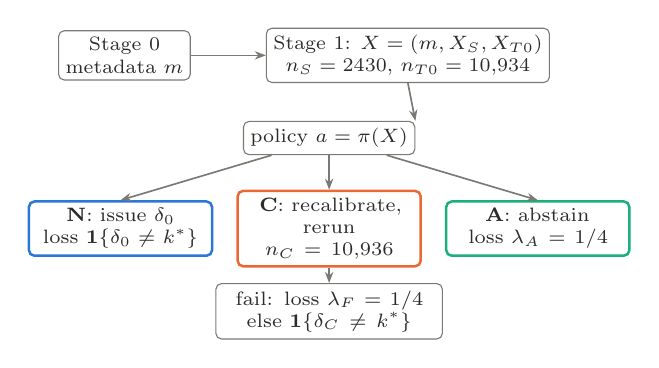
\begin{tikzpicture}[font=\scriptsize,
  box/.style={draw=muted,rounded corners=2pt,align=center,inner sep=2.5pt,text=ink},
  act/.style={box,line width=0.9pt,text width=2.15cm},
  arr/.style={-{Stealth[length=4pt]},muted,line width=0.6pt}]
\node[box] (m) at (-2.6,0) {Stage 0\\metadata $m$};
\node[box] (x) at (1.0,0) {Stage 1: $X=(m,X_S,X_{T0})$\\$n_S=2430$, $n_{T0}=10{,}934$};
\node[box] (pi) at (0,-1.05) {policy $a=\pi(X)$};
\node[act,draw=sN] (N) at (-2.65,-2.2) {\textbf{N}: issue $\delta_0$\\loss $\one\{\delta_0\neq k^*\}$};
\node[act,draw=sC] (C) at (0,-2.2) {\textbf{C}: recalibrate,\\rerun $n_C=10{,}936$};
\node[act,draw=sA] (A) at (2.65,-2.2) {\textbf{A}: abstain\\loss $\lA=1/4$};
\node[box,text width=2.7cm] (C2) at (0,-3.25) {fail: loss $\lF=1/4$\\else $\one\{\delta_C\neq k^*\}$};
\draw[arr] (m)--(x); \draw[arr] (x.south)--(pi.north east);
\draw[arr] (pi)--(N.north); \draw[arr] (pi)--(C); \draw[arr] (pi)--(A.north); \draw[arr] (C)--(C2);
\end{tikzpicture}
\caption{Three-action decision structure under the fixed budget $N=24{,}300$. Every path is charged $N$ shots; on N and A the reserve $n_C$ is charged but unused. Stage-2 randomness on path C is a potential outcome defined on every path (\cref{ass:st2}).}
\label{fig:actions}
\end{figure}

\section{Error and Compilation Model}\label{sec:model}

\paragraph{Compiled-angle model (owner decision D1).} A tagged physical rotation with commanded angle $a$ is executed as $\RZ((1+\eps)a+\phi)$, $\RZ(x)=e^{-ixZ/2}$; every other gate is error-free. In the QAOA cost layer each $\mathrm{RZZ}$ block contains one tagged $\RZ$. The model is synthetic and makes the coherent bias angle-dependent by construction; on hardware whose $Z$ rotations are virtual frame changes it has no direct physical carrier (\cref{sec:hardware}).

\paragraph{Randomized-compiling labels.} Each tagged block is conjugated by a Pauli label $\sigma$, applied without error or tracked virtually, so the commanded angle becomes $a=s\,\theta$ with $s=+1$ for $\sigma\in\{I,Z\}$ and $s=-1$ for $\sigma\in\{X,Y\}$. The labels are drawn uniformly, recorded, and retained.

\begin{lemma}[Frame covariance]\label{lem:frame}
$\sigma\,\RZ((1+\eps)s\theta+\phi)\,\sigma=\RZ((1+\eps)\theta+s\phi)$ exactly. Hence the label-$t$ circuit of candidate $c$ implements the unlabelled circuit with logical angles $u_{c\ell}(t)=(1+\eps)\theta_{c\ell}+s_\ell(t)\phi$, and at $\phi=0$ every label pattern yields the same outcome law.
\end{lemma}
\begin{proof}
$\sigma Z\sigma=sZ$, so $\sigma\RZ(x)\sigma=\RZ(sx)$ with no global phase; apply it with $x=(1+\eps)s\theta+\phi$ and use $s^2=1$.
\end{proof}

The logical error on a tagged angle is therefore $\eps\theta+s\phi$: the multiplicative part is label-blind, and only the additive part is modulated by the label. At $\phi=0$ the label-contrast information for $\eps$ is exactly zero; whether $\eps$ can still be recovered from the label-resolved law depends on what is known about the response, which is the subject of \cref{sec:ident}.

\paragraph{P-amp sensor.} P-amp applies the block $B(a)=\mathrm{CX}\,\RZ((1+\eps)a+\phi)\,\mathrm{CX}$ with control in $|0\rangle$ and target in $|{+}\rangle$, in six repetition and three echo circuits, and measures $\langle X\rangle$ and $\langle Y\rangle$ on the target (18 settings of 135 shots). The phases are linear in $(\eps,\phi)$ with known coefficients, and $(\hat\eps,\hat\phi)$ is their least-squares inversion. A deterministic state-vector check of the 729 circuit--grid cases agrees with this phase model to $3.4\times10^{-15}$, with zero control leakage (post-lock check). Sensor and target share one $(\eps,\phi)$ by construction, so sensor--target transfer cannot fail in this model.

\paragraph{Gap-shift quantity.} For target circuits without labels, write $x=(x_{A},x_{B})$ for the tagged angles of both candidates, $E_j(x_j)=\sum_b s(b)\,|\langle b|U_j(x_j)|{+}^n\rangle|^2$ with a normalised score $s\in[0,1]$, and $g(x)=E_A(x_A)-E_B(x_B)$. The error perturbs $x=\theta$ to $\theta+\delta$ with $\delta_{ji}=\eps\theta_{ji}+\phi$. Let $A=\sum_{j,i}|\theta_{ji}|$ and $M$ the number of tagged rotations. \Cref{thm:B} bounds $|g(\theta+\delta)-g(\theta)|$.

\section{Three-Action Decision Theory}\label{sec:theory}

The theory is sensor-independent and all results are analytic. We give the statements, the assumptions they use, and the derivations the conclusions rest on; full proofs are in \cref{app:theory,app:ident}. Unless a result is marked otherwise, its proof has been checked line by line (\cref{tab:thm} lists the status of every result).

\subsection{Setting}
$\Theta$ is the state space and $k^*:\Theta\to K$ with $K$ finite. Stage-1 evidence $X$ lives in a standard Borel space with law $P_\vt\ll\mu$ and density $p_\vt$.

\begin{assumption}[Evidence]\label{ass:X}
$X$ contains everything the policy may use, including the metadata and $X_{T0}$; $\delta_0$ and the correction estimate are measurable functions of $X$.
\end{assumption}
\begin{assumption}[Policy]\label{ass:pol}
A policy is a measurable $\pi:\mathcal X\to\Delta(\{N,C,A\})$, realised as $a=\alpha(X,U)$ with private randomisation $U$ independent of $(\vt,X,Y)$.
\end{assumption}
\begin{assumption}[Stage 2 as a potential outcome]\label{ass:st2}
For each $\vt$ there is $Y=(F,\delta_C)$, defined on every path and observed only on C, with regular conditional law $Q_\vt(\cdot\mid x)$; $U$ is independent of $(X,Y)$; under D3 the stage-1 allocation does not depend on the action.
\end{assumption}

The action-conditional losses are $l_N(\vt,x)=\one\{\delta_0(x)\neq k^*(\vt)\}$, $l_A=\lA$, and $l_C(\vt,x)=\lF\rho(\vt,x)+c(\vt,x)$ with $\rho=Q_\vt(F{=}1\mid x)$ and $c=Q_\vt(F{=}0,\delta_C\neq k^*\mid x)$.

\subsection{Risk identity and Bayes action}

\begin{theorem}[T1: three-action risk identity]\label{thm:T1}
Under \cref{ass:X,ass:pol,ass:st2}, for every policy $\pi$ and state $\vt$, with $q(\vt)=\E_\vt[l_N]$,
\begin{align}
R(\pi;\vt)&=\E_\vt\bigl[\pi_Nl_N+\pi_Cl_C+\pi_A\lA\bigr]\label{eq:T1a}\\
&=q(\vt)+\E_\vt[\pi_C(l_C-l_N)]+\E_\vt[\pi_A(\lA-l_N)].\label{eq:T1b}
\end{align}
\end{theorem}
\noindent\emph{Derivation.} Condition on $X=x$. The action is $\alpha(x,U)$ and $U\perp Y\mid X$, so the conditional expected loss of path C is $\pi_C(x)[\lF\rho+c]=\pi_C(x)l_C$; paths N and A contribute $\pi_N(x)l_N$ and $\pi_A(x)\lA$ because $l_N$ is a function of $x$. The tower property gives \eqref{eq:T1a}; substituting $\pi_N=1-\pi_C-\pi_A$ gives \eqref{eq:T1b}. Independence is used only in the C term; no independence between $X_S$ and $X_{T0}$ is needed.

\paragraph{Bayes action and pairwise switching.} Fix a prior $\Pi$ and define posterior action risks $\rho_N(x)=e_N(x):=\Pi(\delta_0(x)\neq k^*\mid X=x)$, $\rho_A=\lA$, and $\rho_C(x)=\lF\varphi_F(x)+\bar c(x)$ with $\varphi_F=\E_\Pi[\rho\mid X]$, $\bar c=\E_\Pi[c\mid X]$. Averaging \eqref{eq:T1a} over $\Pi$ gives Bayes risk $\E[\sum_a\pi_a(X)\rho_a(X)]$, minimised pointwise by any $a\in\arg\min_a\rho_a(x)$.

\begin{proposition}[P1: pairwise switching]\label{prop:P1}\status{proved, draft}
The Bayes action prefers A over N iff $e_N(x)>\lA$; C over A iff $\lF\varphi_F(x)+\bar c(x)<\lA$; C over N iff $e_N(x)-\bar c(x)>\lF\varphi_F(x)$. With $a_0$ the best action chosen without looking at $X$, the value of looking at a fixed allocation is $\mathrm{VOI}_{\mathrm{alloc}}=\E[\rho_{a_0}(X)-\min_a\rho_a(X)]\ge0$, with equality iff $a_0$ is Bayes for almost every $x$.
\end{proposition}

So correction can beat issuing only if it lowers the posterior wrong-answer probability by more than the expected failure cost, and it can beat abstaining only if $\lF\varphi_F<\lA$. If one action dominates for almost every $x$, the Bayes policy is fixed and $\mathrm{VOI}_{\mathrm{alloc}}=0$ (P3, \cref{app:theory}); this is the analytic form of the failure mode ``correction benefit has the same sign on every unit''.

\subsection{Reductions}

\begin{corollary}[C1: predecessor's Eq.~(6)]\label{cor:C1}
With $\pi_C\equiv0$, $\lA=0$ and $\pi_A=\one_{\mathrm{Alarm}}$, write $W_f=\{\delta_0\neq k^*\}$, $q_f=P(W_f)$, $d_f=P(\mathrm{Alarm}\cap W_f)$. Then $R=q_f-d_f$, and $R<q_0$ iff $d_f>q_f-q_0$.
\end{corollary}
\noindent\emph{Derivation.} From \eqref{eq:T1b}, $R=q_f+\E[\one_{\mathrm{Alarm}}(0-\one_{W_f})]=q_f-d_f$. The inequality $d_f>q_f-q_0$ is Eq.~(6) of the predecessor project (an alarm is worth having iff it catches more wrong answers than the shots it costs create); C1 shows it is the $C$-free, cost-free slice of T1.

\begin{corollary}[C2: Chow-type reject rule]\label{cor:C2}
Among policies with $\pi_C\equiv0$, the Bayes risk is minimised exactly by abstaining for a.e.\ $x$ with $e_N(x)>\lA$ and issuing for a.e.\ $x$ with $e_N(x)<\lA$ (either on ties).
\end{corollary}
\noindent\emph{Derivation.} The Bayes risk is $\E[e_N(X)]+\E[\pi_A(X)(\lA-e_N(X))]$, minimised pointwise. If $\delta_0$ is the posterior mode, $e_N=1-\max_k\Pi(k\mid x)$ and the rule is ``abstain iff $\max_k\Pi(k\mid x)<1-\lA$'', Chow's rule with threshold $t=\lA$ (equations (2$'$) and (4$'$) of \cite{chow1970}; checked against the published text). With two answers and the posterior mode, $e_N\le1/2$, so abstention is never strictly optimal when $\lA\ge1/2$. In this project N issues the fixed empirical decision, not the posterior mode, so $e_N$ can exceed $1/2$ under coherent bias.

\subsection{Blindness and finite-pilot bounds}

Let $R^*(\vt)=\E_\vt[\min_al_a]$, $D_a=l_a-\min_bl_b\ge0$, $\Reg(\pi;\vt)=R(\pi;\vt)-R^*(\vt)=\E_\vt[\sum_a\pi_aD_a]$, and for a pair $\vt,\vt'$, $\Gamma(x)=\min_a[D_a(\vt,x)+D_a(\vt',x)]$.

\begin{lemma}[L1: action-selection blindness]\label{lem:L1}
If $P_\vt=P_{\vt'}=:P$, then for every policy $\Reg(\pi;\vt)+\Reg(\pi;\vt')\ge\E_P[\Gamma]$, so $\max\{\Reg(\pi;\vt),\Reg(\pi;\vt')\}\ge\tfrac12\E_P[\Gamma]$; and $\Gamma(x)>0$ iff the optimal-action sets at $x$ are disjoint. For any two actions $a_0\neq a_1$, $P_\vt(a\neq a_0)+P_{\vt'}(a\neq a_1)\ge1$.
\end{lemma}

\paragraph{Observation model.} By \cref{ass:X}, $P_\vt=P_{\vt'}$ means equality of the joint law of $(m,X_S,X_{T0})$. L1 therefore applies only to two states of the \emph{same} unit that differ in latent error parameters or response; states with different circuits are never covered. \emph{Two-point construction.} A blindness claim needs a pair $(\vt,\vt')$ with equal stage-1 laws and disjoint optimal actions. \Cref{ex:E1,ex:E2} give the two attempts in this project and their status.

\begin{example}[Single sensed angle; corrected]\label{ex:E1}
If a sensor observes only $\delta_S=\eps a_S+\phi$, the states $(\eps,\phi)$ and $(\eps',\phi+(\eps-\eps')a_S)$ give the same \emph{sensor} law but different gap biases $\eps(a_A-a_B)$ and $\eps'(a_A-a_B)$. L1 needs equal \emph{stage-1} laws, and $X_{T0}$ generally separates the two states. Valid repairs: restrict to policies that use $X_S$ only (L1 applies to the $X_S$-marginal), or keep $X_{T0}$ and use \cref{thm:T2} with the overlap computed on $(X_S,X_{T0})$.
\end{example}

\begin{example}[RC labels at $\phi=0$]\label{ex:E2}\status{conditional; second premise open}
The first premise---two states in the frozen nuisance class with identical label-resolved laws---is discharged by \cref{thm:S1}(2)--(3), provided stage-1 evidence consists only of label-resolved draws of the candidate circuits. The second premise---that the two states imply different optimal actions---is open.
\end{example}

\begin{theorem}[T2: finite-pilot lower bound]\label{thm:T2}
For any pair $\vt_0,\vt_1$ with densities $p_0,p_1$ and any policy:
\begin{align}
&\Reg_0+\Reg_1\ge\textstyle\int\Gamma\min(p_0,p_1)\,d\mu,\label{eq:T2a}\\
&P_0(a\neq a_0)+P_1(a\neq a_1)\ge1-\TV(P_0,P_1)\quad(a_0\neq a_1).\label{eq:T2c}
\end{align}
If $\Gamma\ge\Gamma_{\min}$ a.e.\ on $\{\min(p_0,p_1)>0\}$, then $\max_j\Reg_j\ge\tfrac12\Gamma_{\min}(1-\TV)$. For product laws $P_j^{\otimes}=\bigotimes_{i=1}^nP_{j,i}$,
\begin{align}
1-\TV(P_0^{\otimes},P_1^{\otimes})&\ge\tfrac12\textstyle\prod_i\BC(P_{0,i},P_{1,i})^2,\label{eq:T2e}\\
1-\TV(P_0^{\otimes},P_1^{\otimes})&\ge\tfrac12\exp\bigl(-\textstyle\sum_i\KL_i\bigr),\label{eq:T2d}
\end{align}
with $\KL_i$ taken in either direction, chosen once for all $i$.
\end{theorem}

\paragraph{Constants and direction.} We use $\TV=\tfrac12\int|p_0-p_1|$, so $\int\min(p_0,p_1)=1-\TV$; $\BC=\int\sqrt{p_0p_1}$; and the Hellinger distance $H^2=\int(\sqrt{p_0}-\sqrt{p_1})^2\in[0,2]$, so $\BC=1-H^2/2$. (The Gate~1A artifact stores $\tfrac12\int(\sqrt{p_0}-\sqrt{p_1})^2=1-\BC$ under the name \texttt{hellinger\_squared}.) Both \eqref{eq:T2e} (Le Cam) and \eqref{eq:T2d} (Bretagnolle--Huber) bound the overlap $1-\TV$ from \emph{below} with constant $\tfrac12$, which is the direction an error lower bound needs. The key point for product laws is that $\BC$ multiplies and $\KL$ adds over independent coordinates, whereas $\TV$ does not tensorise: $n\,\TV_1$ is a valid but rapidly vacuous upper bound on $\TV_n$, and ``single-shot TV times $n$'' must not be read as a distance at budget. For an upper bound on $\TV_n$ we also use
\begin{equation}\label{eq:TVup}
\TV(P,Q)\le\sqrt{1-\BC(P,Q)^2}
\end{equation}
(\cref{lem:TVup}, \textsc{proved, draft}). If $P_0(a\neq a_0)+P_1(a\neq a_1)\le\beta<\tfrac12$, then \eqref{eq:T2d} forces $\sum_i\KL_i\ge\log(1/(2\beta))$; for i.i.d.\ shots, $n\ge\log(1/(2\beta))/\min\{\KL(P_0\|P_1),\KL(P_1\|P_0)\}$. T2 bounds wrong-\emph{action} probability, which differs from the estimator-error bounds of \cite{takagi2022,quek2024}.

\subsection{Value of information and collapse}

Let $\Pi$ now be the unit distribution, $\bar R(\pi)=\E_\Pi R(\pi;\vt)$, and the comparator population risks $\bar q_0$ (issue-only, full target), $\bar q_f$ (issue-only, sensor allocation), $\bar r_C$ (always correct), $\lA$; $R_{\mathrm{fix}}=\min\{\bar q_0,\bar q_f,\bar r_C,\lA\}$ and $\DV(\pi)=R_{\mathrm{fix}}-\bar R(\pi)$ at population level.

\begin{assumption}[Comparator consistency]\label{ass:comp}
(a) The sensor-allocation issue-only comparator uses the policy's split and $\delta_0$. (b) Whenever the policy can take C, the always-correct comparator exists and uses the same correction procedure. (c) Population level.
\end{assumption}

\begin{proposition}[D1: value-of-information decomposition]\label{prop:D1}
Under \cref{ass:comp}, $\DV(\pi)=G(\pi)-K$ with $G(\pi)=\E_\Pi\E_\vt[\pi_C(l_N-l_C)+\pi_A(l_N-\lA)]$ and $K=\bar q_f-R_{\mathrm{fix}}\ge0$.
\end{proposition}
\noindent\emph{Derivation.} Averaging \eqref{eq:T1b} over $\Pi$ gives $\bar R(\pi)=\bar q_f-G(\pi)$, so $\DV=G-(\bar q_f-R_{\mathrm{fix}})$; $K\ge0$ because $\bar q_f$ is one of the comparator risks. Hence positive value requires an expected action-loss reduction $G$ larger than the allocation cost $K$ of having set aside sensing and reserve shots. Without allocation (ii), $K$ could be negative and part of $\DV$ could come from allocation alone.

\begin{proposition}[P2: comparator collapse]\label{prop:P2}
Under \cref{ass:comp}, if $\pi$ is information-free---$\pi_a(x)\equiv w_a$ for all $x$, metadata included---then $\DV(\pi)\le0$, with equality iff every action with $w_a>0$ attains $R_{\mathrm{fix}}$.
\end{proposition}
\noindent\emph{Derivation.} With constant weights, \eqref{eq:T1a} gives $\bar R(\pi)=w_N\bar q_f+w_C\bar r_C+w_A\lA$, using \cref{ass:comp}(b) to identify $\E_\Pi\E_\vt l_C$ with $\bar r_C$. Each term is a comparator risk, hence $\ge R_{\mathrm{fix}}$, and so is their convex combination. Two gaps remain and are not covered: metadata-only policies (one option is per-stratum comparators) and finite samples, where comparator mis-selection on development data can make an information-free policy look positive on evaluation data.

\paragraph{Policy non-degeneracy (D2).} A policy is non-degenerate if at least two actions each reach a minimum frequency and the variation is not produced by ties. P2 implies that positive population $\DV$ requires the action to depend on the unit, but not that each action reaches the frequency floor; Gate~4 is an additional requirement, not a consequence of Gate~3.

\section{Sensors and Identifiability}\label{sec:ident}

\subsection{Three notions}
For a model $\{P_{\eps,\eta}\}$ with true point $(\eps_0,\eta_0)$, the \emph{identified set} is $I=\{\eps':\exists\eta',\ P_{\eps',\eta'}=P_{\eps_0,\eta_0}\}$. (i) \emph{Zero efficient information}: the $\eps$-score lies in the closure of the nuisance tangent span---a first-order statement. (ii) \emph{Local non-identification}: $I\cap(\eps_0-r,\eps_0+r)\neq\{\eps_0\}$ for every $r>0$. (iii) \emph{Global non-identification}: $I$ is the whole parameter set. (i) does not imply (ii): for $P_\eps=N(\eps^3,1)$ the information at $\eps_0=0$ is zero, yet $\eps\mapsto\eps^3$ is injective. Every non-identification claim below is therefore proved by an explicit observational equivalence.

\subsection{Nuisance classes}
Observed draws are $(c,t,b)$ with known candidate and label probabilities, so two parameter points are equivalent iff they induce the same family $\{P_{c,t}\}$. By \cref{lem:frame}, $P_{c,t}=R_c(u_c(t))$ with $u_c(t)=(1+\eps)\theta_c+s(t)\phi$. Let $\simp$ be the open simplex on outcomes and $\Sigma_0$ the zero-sum vectors.
\begin{description}
\item[N-free:] $\eta=(R_c)_c$ with $R_c:\R^{L_c}\to\simp$ in a class closed under translation (F1) and under small positivity-preserving bumps (F2); arbitrary, continuous and $C^k$ maps qualify.
\item[N-loc:] $P_{c,t}=q_c+\sum_\ell(\eps\theta_{c\ell}+s_\ell(t)\phi)D_{c\ell}$ with unknown $q_c\in\simp$, $D_{c\ell}\in\Sigma_0$.
\item[N-q:] as N-loc with $D$ known.
\end{description}
N-q $\subseteq$ N-loc, but N-q $\not\subseteq$ N-free (an affine response leaves $\simp$ for large angles), so the classes are not nested. Write $v_c=\sum_\ell\theta_{c\ell}D_{c\ell}$; at $\phi=0$, $P_{c,t}=q_c+\eps v_c$ for every $t$.

\begin{theorem}[Lemma S1$'$]\label{thm:S1}
At any true point with $\phi_0=0$:
\begin{enumerate}[label=(\arabic*)]
\item under N-q, hence under N-loc, $I\supseteq(\eps_0-\delta,\eps_0+\delta)$ with $\delta=m/V>0$, where $m=\min_{c,b}q^0_c(b)$ and $V=\max_c\|v_c\|_\infty$;
\item under N-loc, $I=\R$;
\item under N-free, $I=\R$;
\item if each $R_c$ is differentiable at $(1+\eps_0)\theta_c$, then under N-q, N-loc and N-free the $\eps$-score lies in the nuisance tangent \emph{set}; the efficient information for $\eps$ is $0$.
\end{enumerate}
\end{theorem}
\noindent\emph{Derivation (the constructions).} (1) For $|\eps'-\eps_0|<\delta$ put $q'_c=q^0_c+(\eps_0-\eps')v_c$, $\phi'=0$: it sums to one, stays positive because $|(\eps_0-\eps')v_c(b)|<\delta V=m$, and $q'_c+\eps'v_c=q^0_c+\eps_0v_c$ for every label. (2) For $\eps'\neq0$ rescale $D'=(\eps_0/\eps')D$, $q'=q^0$; for $\eps'=0$ put $q'_c=P_c$, $D'=0$. (3) Translate: $R'_c(u)=R^0_c(u+(\eps_0-\eps')\theta_c)$, $\phi'=0$; then $R'_c((1+\eps')\theta_c)=R^0_c((1+\eps_0)\theta_c)$ for every real $\eps'$, and $R'_c$ keeps the regularity of $R^0_c$. (4) The score $v_c/P_c$ (or $\nabla R_c\theta_c/P_c$) is the score of the in-class nuisance path $q_c+\tau v_c$ (or $R_c+\tau\psi_cw_c$ with a smooth positivity-preserving bump $\psi_c$). Full proofs: \cref{app:ident}.

\begin{proposition}[Sharp identified set under N-q]\label{prop:sharp}
If for some $c$ the map $t\mapsto\sum_\ell s_\ell(t)D^0_{c\ell}$ is non-constant (or $\phi$ is known to be $0$), then $I=(\eps_0-\alpha,\eps_0+\beta)$ with $\alpha=\min_{v_c(b)<0}q^0_c(b)/|v_c(b)|$ and $\beta=\min_{v_c(b)>0}q^0_c(b)/v_c(b)$. If some $v_c\neq0$, both are finite: $\eps$ is locally but \emph{not} globally non-identified.
\end{proposition}

So the three notions really differ here: under N-q the information is zero and identification fails locally, yet the identified set is bounded; under N-loc and N-free it is the whole line.

\begin{corollary}[Profile maximisers]\label{cor:gibbs}
At exact probabilities the profile log-likelihood maximisers attaining the population maximum are exactly $I$ (Gibbs' inequality), even if the class is misspecified. Hence at $\phi_0=0$ the profile maximiser is non-unique in every class above.
\end{corollary}

\paragraph{Shared-response readings (S1$''$).} The frozen class (spec §5.3) treats ``each target context's'' response as unknown, so in the \emph{distinct}-angle design two candidates may share one map $R$. If the class is closed under argument rescaling, $I\supseteq\R\setminus\{-1\}$ (put $R'=R(c\,\cdot)$, $c=(1+\eps_0)/(1+\eps')$); and $-1\in I$ iff all candidate laws coincide, for every $\phi'$ (the evaluation points $s(t)\phi'$ do not depend on the candidate). In the first-order shared version every $\eps'\neq0$ is in $I$, and $0\in I$ iff all candidate laws coincide. Visibility and label-independent offset ($vP+(1-v)o$) only enlarge identified sets (monotonicity). In all six primary designs and every reading, $I$ contains an open interval around $\eps_0$, realised with $\phi'=0$, which lies inside the optimiser box $[-0.05,0.05]^2$ since $|\eps_0|\le0.04$.

\paragraph{From non-uniqueness to Gate~1A FAIL.}\status{specification inference} Spec §7 declares ``a flat profile, nonunique solution \dots\ a failure'' and §9 requires recovery ``at every required grid point''; each design has nine grid points with $\phi=0$. With \cref{cor:gibbs}, Gate~1A fails. This step uses the specification's wording and is not a theorem. Whether readings (a)--(d) exhaust §5.3 is an open specification question.

\subsection{Finite separation at the sensing budget}
The frozen hard pairs are $z_0=(0,0)$ and $z_{1,2}=(\pm0.02,\mp0.02\,\theta_{\mathrm{ref}})$ with $\theta_{\mathrm{ref}}\in\{\pi/8,\pi/4\}$. With $n_S=2430$ i.i.d.\ draws of the joint (label, bitstring) variable, $\BC_n=\BC_1^n$ and $\KL_n=n\KL_1$. Under the \emph{oracle} law (known response), \cref{thm:T2} gives an equal-prior two-point error of at least $0.185$--$0.232$ from $\max\{\tfrac12\BC_n^2,\tfrac12e^{-\KL_n}\}$ (post-lock), and at least $0.245$--$0.366$ from \eqref{eq:TVup} (recomputed from the stored $\BC_n$). Because the oracle law carries at least as much information as any deployable procedure, these bounds hold for every deployable procedure. They are statistical, not action-level: no action map was frozen for these reference contexts. \Cref{fig:lb} shows the three bounds against $n$ for one pair; \cref{tab:pairs} in \cref{app:tables} lists all eight.

\begin{figure}[t]
\centering
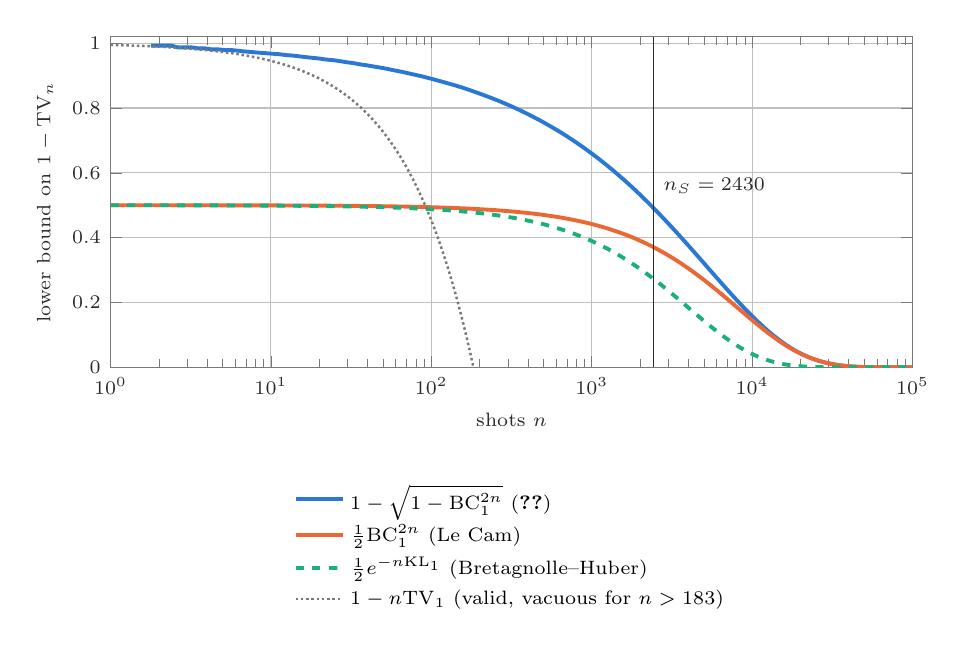
\begin{tikzpicture}
% Data: stored single-shot quantities of the G2-primary pair theta_ref=pi/4, z1=(+0.02,-0.0157):
% results/gate1a/gate1a_results.json -> finite_pairs; ln BC_1 = -6.168566169101564e-05,
% KL_1 = 2.494284712647411e-04, TV_1 = 5.465461558715988e-03. Curves are closed-form transforms.
\begin{axis}[scaffold,scale only axis,width=0.84\columnwidth,height=4.2cm,xmode=log,xmin=1,xmax=1e5,ymin=0,ymax=1.02,
  xlabel={shots $n$},ylabel={lower bound on $1-\TV_n$},samples=120,domain=1:1e5,
  legend style={font=\scriptsize,draw=none,fill=none,at={(0.5,-0.32)},anchor=north,cells={anchor=west},legend columns=1}]
\addplot[sN,smooth] {1-sqrt(1-exp(2*x*(-6.168566169101564e-05)))};
\addlegendentry{$1-\sqrt{1-\BC_1^{2n}}$ (\cref{eq:TVup})}
\addplot[sC,smooth] {0.5*exp(2*x*(-6.168566169101564e-05))};
\addlegendentry{$\tfrac12\BC_1^{2n}$ (Le Cam)}
\addplot[sA,smooth,dashed] {0.5*exp(-x*2.494284712647411e-04)};
\addlegendentry{$\tfrac12 e^{-n\KL_1}$ (Bretagnolle--Huber)}
\addplot[muted,line width=0.9pt,densely dotted,domain=1:183] {1-x*5.465461558715988e-03};
\addlegendentry{$1-n\TV_1$ (valid, vacuous for $n>183$)}
\draw[ink,line width=0.6pt] (axis cs:2430,0) -- (axis cs:2430,1.02) node[pos=0.55,right,font=\scriptsize,text=ink]{$n_S=2430$};
\end{axis}
\end{tikzpicture}
\caption{Product-law lower bounds on the overlap $1-\TV_n$ for the Gate~1A hard pair (G2, $\theta_{\mathrm{ref}}=\pi/4$) under the oracle law. At $n_S=2430$ the overlap is at least $0.49$, so the minimal sum of the two wrong-decision probabilities is at least $0.49$ and the equal-prior error at least $0.245$. Curves are closed-form functions of stored single-shot quantities.}
\label{fig:lb}
\end{figure}

\subsection{Gap-shift bound (Lemma B)}

\begin{theorem}[Lemma B]\label{thm:B}
Assume every tagged angle occurs in exactly one gate (each occurrence of a QAOA angle is its own coordinate) and the error model of \cref{sec:model} acts on tagged rotations only. Then for all $\eps,\phi\in\R$,
\begin{equation}\label{eq:B}
|g(\theta+\delta)-g(\theta)|\le\tfrac12\|\delta\|_1\le\tfrac12\bigl(|\eps|A+|\phi|M\bigr).
\end{equation}
The constant $\tfrac12$ is sharp over this circuit class.
\end{theorem}
\noindent\emph{Derivation.} Fixing all angles but one, $U_j=V_2\RZ(x)V_1$ and $E_j=a+b\cos x+c\sin x$. Since $0\le E_j\le1$ for every $x$, writing $E_j=a+\rho\cos(x-x_0)$ gives $a+\rho\le1$ and $a-\rho\ge0$, so $\rho\le\tfrac12$ and $|\partial E_j/\partial x|\le\tfrac12$ everywhere. Hence $\|\nabla g\|_\infty\le\tfrac12$ on all of $\R^M$, and the fundamental theorem of calculus along $\theta+t\delta$ with Hölder's inequality gives the first inequality; $|\delta_{ji}|\le|\eps||\theta_{ji}|+|\phi|$ gives the second. Sharpness: $E(x)=\cos^2(x/2)$ has $|E'(\pi/2)|=\tfrac12$.

\paragraph{Scope.} The bound is global in $(\eps,\phi)$ and has no remainder term, because the derivative bound holds uniformly along the whole segment; the earlier first-order version of the bound is its linearisation. It is instance-dependent only through $A$ and $M$. A \emph{numerical check} on the frozen populations finds the largest ratio of the actual shift to $\tfrac12B$ to be $0.431$ (Gate~2) and $0.213$ (Gates~3--4). It says nothing about the plug-in $\hat B=B(\hat\eps,\hat\phi)$, its coverage, shot noise in $\hat g_0$, decision-flip probabilities, or models beyond the noiseless compiled-angle model. $\hat B$ is therefore a heuristic alarm threshold built from a provable population bound, not a guarantee about the rule.

\subsection{P-amp identifiability (Gate~1B basis)}
With its own known reference, P-amp observes phases that are linear in $(\eps,\phi)$ with a rank-two design, so $(\eps,\phi)$ is identified at every grid point and noiseless recovery is exact (81/81 grid points within $10^{-8}$). The resource condition compares the conservative standard error $\mathrm{SE}(\hat\eps)=0.0070902$ (from the frozen bound $\mathrm{Var}(\hat u)\le1/135$ per setting at visibility $v=1$) with the frozen threshold $0.0071429$: a margin of $1-0.0070902/0.0071429=0.74\%$. Since the standard error scales as $1/v$, the condition fails for $v<0.0070902/0.0071429=0.99263$. Visibility loss was not modelled in any gate.

\begin{figure}[t]
\centering
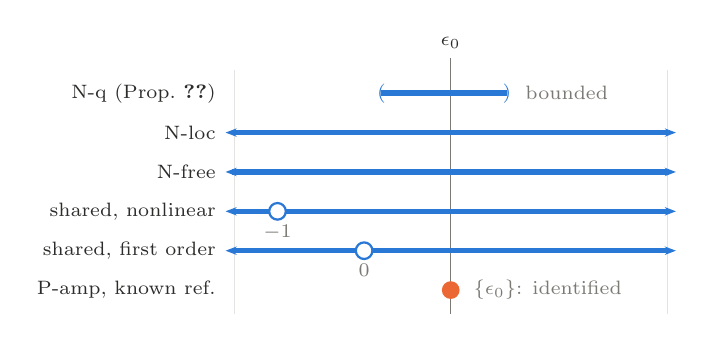
\begin{tikzpicture}[font=\scriptsize,x=0.55cm,y=0.5cm]
% Schematic (no data): identified set for epsilon at phi_0=0 under each nuisance class (Thm. S1', Prop. sharp, S1'').
\def\row#1#2{\node[anchor=east,text=ink,align=right] at (-0.2,#1) {#2};}
\foreach \y/\lab in {0/{N-q (Prop.~\ref{prop:sharp})},-1/{N-loc},-2/{N-free},-3/{shared, nonlinear},-4/{shared, first order},-5/{P-amp, known ref.}}{\row{\y}{\lab}}
\draw[grid,line width=0.4pt] (0,0.6) -- (0,-5.6); \draw[grid,line width=0.4pt] (10,0.6) -- (10,-5.6);
\draw[muted] (5,0.9) node[above,text=ink]{$\eps_0$} -- (5,-5.6);
\draw[sN,line width=2pt] (3.4,0) -- (6.3,0); \node[sN,font=\scriptsize] at (3.4,0) {(}; \node[sN,font=\scriptsize] at (6.3,0) {)};
\node[anchor=west,text=muted] at (6.5,0) {bounded};
\draw[sN,line width=2pt,-{Stealth[length=4pt]}] (5,-1) -- (10.2,-1); \draw[sN,line width=2pt,-{Stealth[length=4pt]}] (5,-1) -- (-0.2,-1);
\draw[sN,line width=2pt,-{Stealth[length=4pt]}] (5,-2) -- (10.2,-2); \draw[sN,line width=2pt,-{Stealth[length=4pt]}] (5,-2) -- (-0.2,-2);
\draw[sN,line width=2pt,-{Stealth[length=4pt]}] (5,-3) -- (10.2,-3); \draw[sN,line width=2pt,-{Stealth[length=4pt]}] (5,-3) -- (-0.2,-3);
\fill[white] (1.0,-3) circle (3pt); \draw[sN,line width=0.8pt] (1.0,-3) circle (3pt); \node[below,text=muted] at (1.0,-3.1) {$-1$};
\draw[sN,line width=2pt,-{Stealth[length=4pt]}] (5,-4) -- (10.2,-4); \draw[sN,line width=2pt,-{Stealth[length=4pt]}] (5,-4) -- (-0.2,-4);
\fill[white] (3.0,-4) circle (3pt); \draw[sN,line width=0.8pt] (3.0,-4) circle (3pt); \node[below,text=muted] at (3.0,-4.1) {$0$};
\fill[sC] (5,-5) circle (3.2pt); \node[anchor=west,text=muted] at (5.3,-5) {$\{\eps_0\}$: identified};
\end{tikzpicture}
\caption{Identified set for $\eps$ at a $\phi_0=0$ grid point. Retained RC labels (rows 1--5; Gate~1A): local non-identification in every class, global under N-loc and N-free, bounded under N-q; open circles mark the single excluded point when candidate laws differ. Efficient information is zero in all five rows. P-amp with its own known reference (row 6; Gate~1B) identifies $\eps$. Schematic; not to scale.}
\label{fig:ident}
\end{figure}

\section{Experimental Design}\label{sec:design}

\paragraph{Gate sequence and locks.} Gates were run in a fixed order with a stopping rule (\cref{fig:flow}). Each gate's design document was committed with a SHA-256 manifest before the run, and the runner refused to run unless the repository was at the lock commit.

\paragraph{Evidence boundary.} Every gate result (\cref{sec:results,sec:failure}) comes from shot-noise-only simulation of the synthetic compiled-angle model on 2--6 qubits at QAOA depth one; no device, decoherence, visibility loss, or drift is modelled. The hardware pilot of \cref{sec:hardware} is a separate study with its own lock and does not enter any gate verdict. The gate locks are internal Git and SHA-256 locks without an independent timestamp, so we call the gates prespecified rather than preregistered, and the analysis code was not itself locked (\cref{sec:failure}). Where a quantity was computed after a gate result, it is labelled \emph{post-lock}; such analyses can qualify a verdict but cannot change it. Label definitions are collected in \cref{tab:labels}.

\begin{figure*}[t]
\centering
\begin{tikzpicture}[font=\scriptsize,node distance=5mm and 7mm,
  g/.style={draw=muted,rounded corners=2pt,align=center,inner sep=3pt,text=ink,minimum height=11mm,text width=24mm},
  pass/.style={g,draw=sN,line width=0.9pt},fail/.style={g,draw=sC,line width=0.9pt},
  skip/.style={g,draw=ref,dashed,text=muted},
  arr/.style={-{Stealth[length=4pt]},muted,line width=0.6pt}]
\node[g] (m) {M1--M2\\contract, theory,\\E2 and RC semantics};
\node[fail,right=of m] (g1a) {\textbf{Gate 1A: FAIL}\\RC labels\\(Thm.~\ref{thm:S1}, spec §7/§9)};
\node[pass,right=of g1a] (g1b) {\textbf{Gate 1B: PASS}\\P-amp, noiseless,\\0.7\% margin};
\node[pass,right=of g1b] (g2) {\textbf{Gate 2: formal PASS}\\precision 0.093\\vs base 0.077};
\node[fail,right=of g2] (g3) {\textbf{Gate 3: FAIL}\\$\DV=0.0000804$\\LB $-0.000743$};
\node[g,below=6mm of g3] (g4) {Gate 4: PASS\\(moot)};
\node[g,below=6mm of g2,draw=ink,line width=0.9pt] (stop) {\textbf{stop after M6}\\$\rightarrow$ MT7 synthesis};
\node[skip,below=6mm of g1b] (m7) {M7 registration,\\holdout: not run};
\draw[arr] (m)--(g1a); \draw[arr] (g1a)--node[above]{route}(g1b); \draw[arr] (g1b)--(g2); \draw[arr] (g2)--(g3);
\draw[arr] (g3)--(g4); \draw[arr] (g4)--(stop); \draw[arr,dashed] (stop)--(m7);
\end{tikzpicture}
\caption{Gate route and stopping path. Blue outline: pass; orange outline: fail. Gate~1A's failure routed to the prespecified fallback sensor (Gate~1B). Gate~3's failure triggered the frozen stop rule; Gate~4 passed its frequency rule but is moot.}
\label{fig:flow}
\end{figure*}

\paragraph{Gate 1 (M3 lock).} Exact enumeration on the 2-qubit edge (G2) and 3-qubit path (G3) at $p=1$, $\beta=\pi/8$, in three designs each (single angle $\pi/4$; same pair $(\pi/4,\pi/4)$; distinct pair $(\pi/8,\pi/4)$), 16 two-qubit Pauli labels per tagged block, all joint label vectors retained, a $9\times9$ grid $\eps,\phi\in\{0,\pm0.005,\pm0.01,\pm0.02,\pm0.04\}$, and $n_S=2430$. Information sources were kept separate: I1 (label contrast, response unknown), I2 (oracle, known response; diagnostic only), I3 (deployable profile information under the §5.3 class). Gate~1A required, in at least one design, rank two for I1 plus admissible I3, exact recovery at every grid point by profile maximum likelihood from nine starts in the box $[-0.05,0.05]^2$, and agreement of all controls. Gate~1B (fallback) required rank two, noiseless recovery, the resource condition, and no phase ambiguity.

\paragraph{Gate 2 (development).} 6600 units from 10 graph strata on 2--5 qubits (edge-2, path-3, triangle-3, path-4, cycle-4, star-4, complete-4, path-5, cycle-5, star-5), four mixer angles $\beta\in\{\pi/16,\pi/8,3\pi/16,\pi/4\}$, 11 candidate pairs, and 15 error points; 4905 evaluable, split 1179/3726 into rule development and evaluation. The frozen rule predicts positive correction benefit exactly when the P-amp estimate is defined and unambiguous, either parameter clears its two-sided $1.96$-standard-error threshold, $\hat g_0\neq0$, and $|\hat g_0|\le\hat B$. The baseline predicts the constant majority class. The metric is balanced accuracy; the gate passes if the full improvement is positive and the minimum leave-one-graph-out improvement is at least $0.05$.

\paragraph{Gates 3--4 (development, split-99).} 99 connected graph clusters on 4--6 qubits generated deterministically from SHA-256 edge masks; clusters 0--32 form the policy-lock/power partition and 33--98 the evaluation partition; 60 contexts per graph (four $\beta$, three $\gamma$-pairs, five error points), 5940 units, 3545 evaluable evaluation units in 66 clusters. The deployable policy is ordered: C if the Gate-2 correction predicate holds; else A if P-amp is undefined or ambiguous or $|\hat g_0|\le1.96\,\mathrm{SE}_{g_0}$; else N. The fixed comparator was selected once on the 33 policy-lock clusters. Gate~3 passes only if $\DV>0$ and the one-sided 95\% lower bound---the 5th percentile of 10{,}000 cluster-bootstrap means of the 66 cluster means of $\Delta_u$---is strictly positive. Gate~4 passes if at least two actions occur on $\ge5\%$ of units and in $\ge10$ of 66 clusters. Power was estimated from 5000 resampled 66-cluster studies of the policy-lock cluster means with the approximation $\text{mean}-1.669\,\mathrm{SD}/\sqrt{66}$.

\paragraph{Scoring.} Shots are multinomial draws (NumPy PCG64) with seeds derived from SHA-256 unit keys. Action losses are 256-replicate Monte Carlo estimates of selection probabilities and are used only for scoring, never as policy inputs.

\section{Results}\label{sec:results}

The four gates answer the three questions of \cref{sec:intro} in turn: can the evidence identify the error (Gates~1A and 1B), does it single out the units that benefit from correction (Gate~2), and does acting on it beat the best fixed policy (Gates~3 and 4)?

\subsection{Gate 1A: FAIL}
The verdict rests on the analysis of \cref{sec:ident}, not on the frozen run's report, whose I3, recovery, and control entries were hard-coded rather than computed: \cref{thm:S1,cor:gibbs} and S1$''$ show that the profile maximiser is non-unique at the nine $\phi=0$ points of every design and every reading, and the specification turns this into FAIL. A post-lock computation confirms zero efficient information for $\eps$ at $\phi=0$ (largest value $6.8\times10^{-21}$ per shot), while the oracle information at the same points is $0.24$--$0.62$ per shot: labels are not uninformative when the response is known, which is why the result must not be read as ``RC labels cannot sense $\eps$''. The frozen nuisance class is ambiguous; under its literal first-order reading, the G3 designs retain a second-order signal of at most $3.5\times10^{-6}$ per shot at $\phi\neq0$, giving $\mathrm{SE}(\hat\eps)\gtrsim11$ at budget.

\subsection{Gate 1B: PASS in the synthetic known-reference model}
The design had rank two, recovered $(\eps,\phi)$ within $10^{-8}$ at all 81 grid points, showed no phase ambiguity, and met the resource condition with a 0.7\% margin; a post-lock state-vector check confirmed the circuit semantics. Robustness to visibility loss was not tested (\cref{sec:failure}).

\subsection{Gate 2: formal PASS, practical conclusion narrowed}
The frozen rule had balanced accuracy $0.5871$ against $0.5000$, full improvement $0.0871$, and leave-one-graph-out minimum $0.0658\ge0.05$. The reading we adopt is:
\begin{quote}\small
Gate~2 formally passed its prespecified, internally locked rule, but the diagnostic did not demonstrate useful selective prediction of which units benefit from correction. Its precision was 0.093 versus a base rate of 0.077, and much of the apparent gain came from excluding large-gap units. Therefore Gate~2 is retained as a formal PASS but not interpreted as evidence of operationally useful benefit selection.
\end{quote}
The rule predicted benefit on 78.7\% of evaluation units (sensitivity $0.948$, specificity $0.227$). The gap-bound condition alone reaches balanced accuracy $0.596$, higher than the full rule; the oracle indicator ``$(\eps,\phi)\neq0$'' reaches only $0.512$ (\cref{fig:gate2}; post-lock, exploratory). Of 287 positive labels, 126 lie within two Monte Carlo standard deviations of zero. The same-budget P2 comparator (balanced accuracy $0.522$) is structurally blind on 3300 of 6600 units because its rounding rule turns the twin mixer into the identity for $\beta\in\{\pi/16,\pi/8\}$.

\begin{figure}[t]
\centering
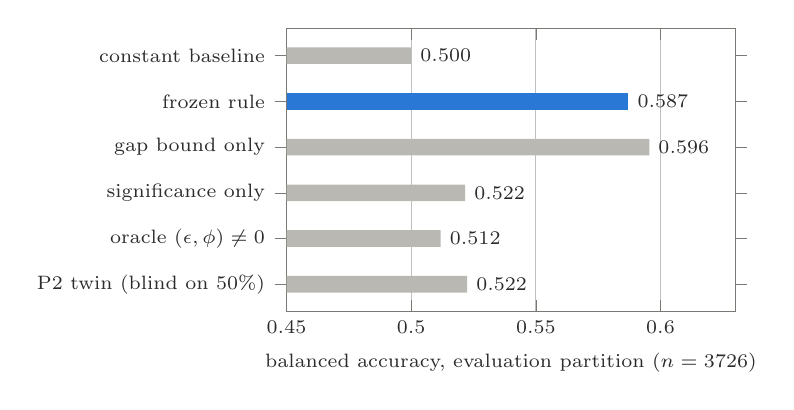
\begin{tikzpicture}
% Data: results/dev/gate2_results.json (frozen rule, baseline) and results/errata/gate2_diagnostics.json (post-lock).
\begin{axis}[scaffold,scale only axis,width=0.47\columnwidth,height=3.6cm,xbar,bar width=6pt,bar shift=0pt,xmin=0.45,xmax=0.63,xticklabel style={/pgf/number format/fixed,/pgf/number format/precision=2},
  symbolic y coords={base,rule,gap,sig,oracle,ptwo},ytick={base,rule,gap,sig,oracle,ptwo},
  yticklabels={constant baseline,frozen rule,gap bound only,significance only,{oracle $(\eps,\phi)\neq0$},P2 twin (blind on 50\%)},
  y dir=reverse,xlabel={balanced accuracy, evaluation partition ($n=3726$)},ymajorgrids=false,xmajorgrids,
  nodes near coords,nodes near coords style={font=\scriptsize,text=ink,/pgf/number format/fixed,/pgf/number format/fixed zerofill,/pgf/number format/precision=3},
  enlarge y limits=0.12,every axis plot/.append style={line width=0pt}]
\addplot[fill=ref,draw=none] coordinates {(0.500,base) (0.5955,gap) (0.5216,sig) (0.5118,oracle) (0.5224,ptwo)};
\addplot[fill=sN,draw=none] coordinates {(0.5871,rule)};
\end{axis}
\end{tikzpicture}\\[1mm]
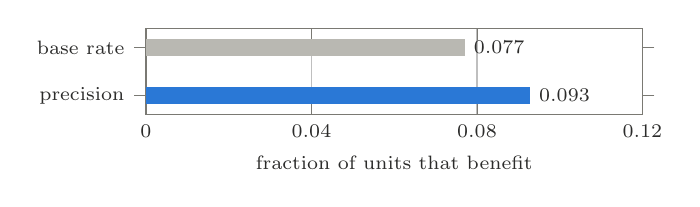
\begin{tikzpicture}
\begin{axis}[scaffold,scale only axis,width=0.52\columnwidth,height=1.1cm,xbar,bar width=6pt,bar shift=0pt,xmin=0,xmax=0.12,xtick={0,0.04,0.08,0.12},xticklabel style={/pgf/number format/fixed,/pgf/number format/precision=2},
  symbolic y coords={base rate,precision},ytick={base rate,precision},y dir=reverse,xlabel={fraction of units that benefit},ymajorgrids=false,xmajorgrids,
  nodes near coords,nodes near coords style={font=\scriptsize,text=ink,/pgf/number format/fixed,/pgf/number format/fixed zerofill,/pgf/number format/precision=3},
  enlarge y limits=0.4,every axis plot/.append style={line width=0pt}]
\addplot[fill=ref,draw=none] coordinates {(0.0770,base rate)};
\addplot[fill=sN,draw=none] coordinates {(0.0928,precision)};
\end{axis}
\end{tikzpicture}
\caption{Gate~2. Top: the frozen rule beats the constant baseline, but the gap-bound condition alone does slightly better, and the oracle error indicator barely beats the baseline---the gain comes from excluding large-gap units, not from detecting who benefits. Bottom: among predicted-positive units, 9.3\% benefit, against 7.7\% overall. Diagnostics other than the frozen rule and baseline are post-lock and exploratory.}
\label{fig:gate2}
\end{figure}

\subsection{Gate 3: FAIL}
On the 33 policy-lock clusters, always-correct had mean loss $0.007914$, against $0.029243$ (N-full), $0.029577$ (N-sensor-allocation), and $0.25$ (A-always), and was selected. On the 66 evaluation clusters, $\DV=0.0000804$ with one-sided 95\% lower bound $-0.000743$: FAIL. The frozen N-path loss ignored selection on the same shots (\cref{sec:estimand}); a post-lock reanalysis with the conditional loss gives $\DV=0.000237$ and lower bound $-0.000625$. Being post-lock, it cannot change the verdict. Estimated power was $0.0004$; the minimum detectable mean was $0.000665$, against a policy-lock mean of $-0.00063$ (\cref{fig:gate3}).

\begin{figure}[t]
\centering
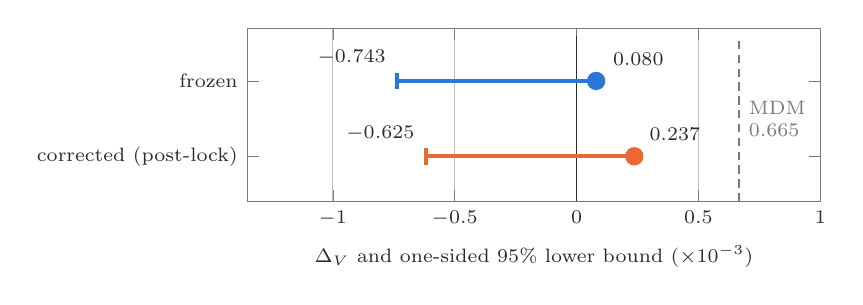
\begin{tikzpicture}
% Data: results/gate34/gate34_results.json (frozen dV, LB, MDM) and results/errata/gate34_estimand.json (corrected; post-lock).
% Units: 1e-3 loss.
\begin{axis}[scaffold,scale only axis,width=0.6\columnwidth,height=2.2cm,xmin=-1.35,xmax=1.0,ymin=0.4,ymax=2.7,ytick={1,2},
  yticklabels={corrected (post-lock),frozen},ymajorgrids=false,xmajorgrids,xlabel={$\DV$ and one-sided 95\% lower bound ($\times10^{-3}$)},
  every axis plot/.append style={line width=1.4pt}]
\draw[ink,line width=0.6pt] (axis cs:0,0.4)--(axis cs:0,2.6);
\draw[muted,densely dashed,line width=0.8pt] (axis cs:0.665,0.4)--(axis cs:0.665,2.6) node[pos=0.5,right,font=\scriptsize,text=muted,align=left]{MDM\\0.665};
\addplot[sN,-{Bar[width=6pt]}] coordinates {(0.0804,2) (-0.743,2)};
\addplot[sN,only marks,mark=*,mark size=2.6pt] coordinates {(0.0804,2)};
\addplot[sC,-{Bar[width=6pt]}] coordinates {(0.2369,1) (-0.6249,1)};
\addplot[sC,only marks,mark=*,mark size=2.6pt] coordinates {(0.2369,1)};
\node[font=\scriptsize,text=ink,anchor=south west] at (axis cs:0.11,2.08) {0.080};\node[font=\scriptsize,text=ink,anchor=south east] at (axis cs:-0.743,2.08) {$-0.743$};
\node[font=\scriptsize,text=ink,anchor=south west] at (axis cs:0.26,1.08) {0.237};\node[font=\scriptsize,text=ink,anchor=south east] at (axis cs:-0.625,1.08) {$-0.625$};
\end{axis}
\end{tikzpicture}\\[1mm]
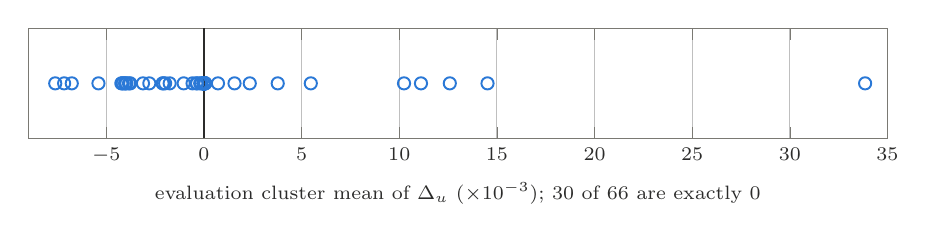
\begin{tikzpicture}
% Data: the 66 frozen evaluation cluster means of Delta_u, results/gate34/gate34_results.json -> gate3.cluster_means (x1e-3).
\begin{axis}[scaffold,scale only axis,width=0.9\columnwidth,height=1.4cm,xmin=-9,xmax=35,ymin=-1,ymax=1,ytick=\empty,ymajorgrids=false,xmajorgrids,
  xlabel={evaluation cluster mean of $\Delta_u$ ($\times10^{-3}$); 30 of 66 are exactly 0}]
\addplot[only marks,mark=o,mark size=2.2pt,sN,line width=0.7pt] coordinates {
(0,0)(0,0)(14.518,0)(0,0)(0,0)(-7.161,0)(0,0)(33.854,0)(0,0)(0,0)(-0.347,0)(-0.130,0)(0,0)(0,0)(-4.036,0)(0,0)(0,0)(-4.167,0)(0,0)(0,0)(3.776,0)(-2.799,0)(0,0)(-6.771,0)(-1.042,0)(0,0)(-0.195,0)(1.563,0)(11.111,0)(-4.036,0)(0,0)(0,0)(0.065,0)(0,0)(0,0)(-1.989,0)(0,0)(2.344,0)(-4.232,0)(-2.121,0)(-2.083,0)(-4.167,0)(0,0)(-1.758,0)(-3.971,0)(0,0)(-5.404,0)(-0.391,0)(0,0)(10.243,0)(0,0)(-3.125,0)(0,0)(-3.776,0)(-0.586,0)(12.587,0)(0,0)(0,0)(0.716,0)(5.469,0)(0,0)(-7.617,0)(-3.841,0)(0,0)(0,0)(0.065,0)};
\draw[ink,line width=0.6pt] (axis cs:0,-1)--(axis cs:0,1);
\end{axis}
\end{tikzpicture}
\caption{Gate~3. Top: point estimates and one-sided 95\% cluster-bootstrap lower bounds; both bounds are negative and both point estimates lie below the minimum detectable mean of the design. Bottom: the 66 evaluation cluster means (frozen); most clusters show no difference because the policy coincides with always-correct, and a few clusters with large values dominate the mean.}
\label{fig:gate3}
\end{figure}

\paragraph{Where $\DV$ comes from.} On C units the policy's loss equals the selected comparator's loss exactly (the same corrected rerun), so C units contribute $0$. Recomputing from the stored per-unit records decomposes the frozen $\DV=0.0000804$ into $-0.000260$ from the 919 N units and $+0.000340$ from the 53 A units; the corrected estimand changes only the N term, to $-0.000104$. On the A units always-correct averaged $0.273$, slightly worse than abstaining ($0.25$); on the N units issuing averaged $0.0028$ (frozen) against $0.0018$ for always-correct.

\subsection{Gate 4: PASS, moot}
N was chosen on 25.9\% of units in all 66 clusters, C on 72.6\% in all 66, A on 1.5\% in 29 (\cref{fig:gate4}). Two actions clear both thresholds, so Gate~4 passes, but it is moot after Gate~3. The thresholds were fixed a priori rather than derived from power. One observed tie took the frozen abstain branch.

\begin{figure}[t]
\centering
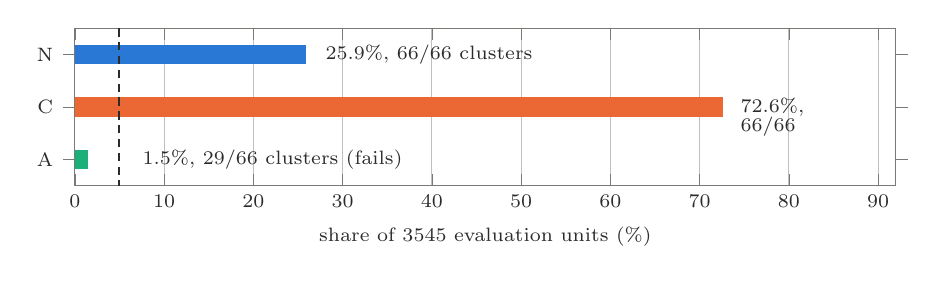
\begin{tikzpicture}
% Data: results/gate34/gate34_results.json -> gate4.actions (frozen).
\begin{axis}[scaffold,scale only axis,width=0.86\columnwidth,height=2.0cm,xbar,bar width=7pt,bar shift=0pt,xmin=0,xmax=92,
  symbolic y coords={N,C,A},ytick={N,C,A},y dir=reverse,xlabel={share of 3545 evaluation units (\%)},ymajorgrids=false,xmajorgrids,
  enlarge y limits=0.25,every axis plot/.append style={line width=0pt}]
\addplot[fill=sN,draw=none] coordinates {(25.92,N)};
\addplot[fill=sC,draw=none] coordinates {(72.58,C)};
\addplot[fill=sA,draw=none] coordinates {(1.50,A)};
\draw[ink,densely dashed,line width=0.7pt] (axis cs:5,{[normalized]-0.5})--(axis cs:5,{[normalized]2.5});
\node[font=\scriptsize,text=ink,anchor=west] at (axis cs:27,N) {25.9\%, 66/66 clusters};
\node[font=\scriptsize,text=ink,anchor=west] at (axis cs:73.5,C) {72.6\%,};
\node[font=\scriptsize,text=ink,anchor=west] at (axis cs:6.5,A) {1.5\%, 29/66 clusters (fails)};
\node[font=\scriptsize,text=ink,anchor=north west] at (axis cs:73.5,C) {66/66};
\end{axis}
\end{tikzpicture}
\caption{Gate~4 action frequencies. Dashed line: the frozen 5\% floor (a second floor requires presence in $\ge10$ of 66 clusters). N and C clear both; A does not. The policy coincides with always-correct on 72.6\% of units, which is why $\DV$ is so small.}
\label{fig:gate4}
\end{figure}

\subsection{Stop}
Under the frozen stopping rule, the Gate~3 failure ended the study after milestone M6; no confirmatory run followed.

\section{Failure Analysis}\label{sec:failure}

\paragraph{Why Gate~3 is null.} D1 says $\DV=G-K$. With always-correct selected, $R_{\mathrm{fix}}=\bar r_C$, and the policy can add value only on units where it deviates from C and the deviation lowers loss. In this model always-correct is already near-optimal (policy-lock loss $0.0079$ against $0.029$ for issue-only), so $G$ is bounded by small per-unit differences on the 27\% of units where the policy deviates; on the N units deviating from C was harmful on average, and on the A units it helped slightly. This is the empirical counterpart of P3: when one action nearly dominates for almost every $x$, the value of looking is nearly zero. We offer it as an explanation, not as a tested finding.

\paragraph{Why Gate~2 is not selectivity.} Balanced accuracy against a constant baseline rewards any statistic associated with the label. The gain comes from the gap-bound condition, which removes large-gap units where no-action accuracy is already about one; detecting that an error is present adds almost nothing. The labels are also noisy and measure unconditional unit-level benefit, not the decision-time quantity that Gate~3 scores. The Gate~2 lock also lacked the uncertainty bound and power analysis that the program plan requested, and its margin rationale concerns resolution, not relevance.

\paragraph{The Gate~1B margin.} The resource condition passes with 0.74\% headroom at visibility one and fails for any visibility below $0.99263$. The pass therefore concerns an idealised sensor; on hardware it does not (\cref{sec:hardware}).

\subsection{Frozen versus corrected Gate~3 estimand}\label{sec:estimand}
For a fixed unit let $W=\{\delta_0\neq k^*\}$ be the event that the issued answer is wrong, $\one_N$ the event that the policy chooses N, and $q=P(W)$ the unconditional always-issue error, which is a unit-level constant. The policy's true expected N-path loss is $\E[\one_N\one_W]=P(N\cap W)$ (T1, $l_N$). The frozen runner instead scored $\E[\one_N(1-p_{\mathrm{correct}})]=P(N)\,q$. Their difference is
\begin{equation}\label{eq:cov}
\begin{aligned}P(N)\,q-P(N\cap W)&=-\bigl(P(N\cap W)-P(N)P(W)\bigr)\\&=-\mathrm{Cov}(\one_N,\one_W)\end{aligned}
\end{equation}
(\textsc{proved, draft}; \cref{app:estimand}). The policy chooses N only when $|\hat g_0|>1.96\,\mathrm{SE}_{g_0}$, an event computed from the same shots as $\delta_0$, and conditional on a large observed gap the issued answer is less often wrong; so $\mathrm{Cov}(\one_N,\one_W)\le0$ is expected and the frozen N-path loss is biased upward. The stored records agree: mean N-path loss $0.00278$ (frozen, unconditional) against $0.00218$ (realised, conditional) on the 919 N units. The correction raises $\DV$ by $0.000156$ but leaves its lower bound negative.

\paragraph{Governance defects.} (i) The Gate~1A runner wrote its verdict, I3 ranks, recovery, and control statuses as literals. (ii) Analysis code was outside every lock. (iii) Power was computed in the same execution as the evaluation, so no decision point existed between them; had it been inspected first, the design could have been revised. (iv) Locks state ``owner-approved'' without review notes, and lock-to-run intervals were 2--34 minutes. (v) Selection probabilities were estimated with 256 replicates (granularity $1/256$) although exact values were computable, which is coarse relative to $|\DV|<0.001$. (vi) Gate~4 thresholds were not power-derived, and 25.7\% of Gate~2 units were exact ideal-gap ties, not prescreened. None of these changes a verdict; all limit what the locks prove. Each is documented in the errata listed in \cref{tab:frozen}.

\section{A Hardware Pilot of the Sensor}\label{sec:hardware}

Gate~1B passed with 0.74\% headroom at visibility one, and the resource condition fails for any visibility below $0.99263$ (\cref{sec:ident}). Whether a real processor keeps the sensor within that standard is therefore the first question to ask of hardware. We answered it in a separately locked pilot (HW-P1, Stage~A); it does not revisit any gate verdict.

\subsection{Design}
\paragraph{Injected rather than native error.} On IBM processors $Z$ rotations are virtual frame changes \cite{mckay2017vz}: they are applied without error and without duration, so the compiled-angle error of \cref{sec:model} cannot arise physically on an $\RZ$. The pilot therefore \emph{injects} it: each tagged rotation in the P-amp circuits is compiled as $\RZ((1+\eps)a+\phi)$ with known $(\eps,\phi)$, which the estimator never sees. This changes the estimand. The pilot measures how precisely and how accurately P-amp recovers a known compiled-angle perturbation under real noise; it says nothing about whether such an error occurs naturally.

\paragraph{Execution plan.} One Heron-family processor, \texttt{ibm\_marrakesh}, with physical qubits 53 (target) and 54 (control), chosen before execution as the pair minimising the sum of the two readout errors and the CZ error in the calibration snapshot; fractional gates were disabled. The five injected points were the Gate~3--4 error grid, $(0,0)$, $(\pm0.02,0)$, $(0.04,0.01)$ and $(-0.04,-0.01)$. Each estimate used the frozen 18 settings of 135 shots, 2430 shots in all. Eight blocks were run in sequence; each contained all five points in a seeded random order, one phase-blind control per point (P-amp measured in the $Z$ basis), and four readout-calibration circuits, for 134{,}600 shots in total. Circuits were transpiled at optimisation level~1 with barriers around each tagged block, with dynamical decoupling and twirling off; unmitigated counts are the primary analysis. The protocol, code, environment, seeds, and command were hashed in a lock committed before the first job (about two minutes earlier); execution was gated on that hash, and the written approval record was added afterwards. There was no external timestamp, so the pilot is prespecified under an internal lock, not preregistered.

\subsection{Results}
All eight blocks completed on one calibration snapshot, using 56 QPU-charge seconds. The validity checks passed: readout assignment error was 0.8--1.7\% per block, the phase-blind controls showed no dependence on the injected point ($|z|\le0.60$ against a Bonferroni threshold of 2.50), and the zero-injection estimate drifted by $0.0001$ per block. \Cref{tab:hw} and \cref{fig:hw} summarise the estimates.

\begin{table*}[t]
\centering\footnotesize\setlength{\tabcolsep}{5pt}
\caption{HW-P1 Stage A on \texttt{ibm\_marrakesh} (qubits 53/54), eight blocks of 2430 shots per point, unmitigated. Bias and visibility are from the locked analysis; the precision column is the standard deviation of one 2430-shot estimate (post-lock correction, see text), with a 95\% block-bootstrap interval. The frozen precision threshold is $0.0071429$.}\label{tab:hw}
\begin{tabular}{@{}lrrrrrl@{}}
\toprule
Injected $(\eps,\phi)$ & mean $\hat\eps$ & $\eps$ bias (95\% CI) & $\phi$ bias & SD of one estimate (95\% CI) & visibility & precision label \\
\midrule
$(0,0)$ & $-0.0128$ & $-0.0128$ $[-0.0166,-0.0086]$ & $+0.0091$ & $0.0062$ $[0.0026,0.0082]$ & 0.955 & inconclusive \\
$(+0.02,0)$ & $+0.0166$ & $-0.0034$ $[-0.0069,+0.0006]$ & $+0.0076$ & $0.0059$ $[0.0023,0.0072]$ & 0.955 & inconclusive \\
$(-0.02,0)$ & $-0.0210$ & $-0.0010$ $[-0.0049,+0.0019]$ & $+0.0086$ & $0.0053$ $[0.0013,0.0072]$ & 0.951 & inconclusive \\
$(+0.04,+0.01)$ & $+0.0322$ & $-0.0078$ $[-0.0126,-0.0029]$ & $+0.0075$ & $0.0077$ $[0.0031,0.0101]$ & 0.957 & inconclusive \\
$(-0.04,-0.01)$ & $-0.0460$ & $-0.0060$ $[-0.0138,+0.0011]$ & $+0.0094$ & $0.0117$ $[0.0057,0.0146]$ & 0.948 & inconclusive \\
\midrule
pooled (35 d.f.) & & & & $0.0077$ $[0.0052,0.0084]$ & & inconclusive \\
\bottomrule
\end{tabular}
\end{table*}

\begin{figure}[t]
\centering
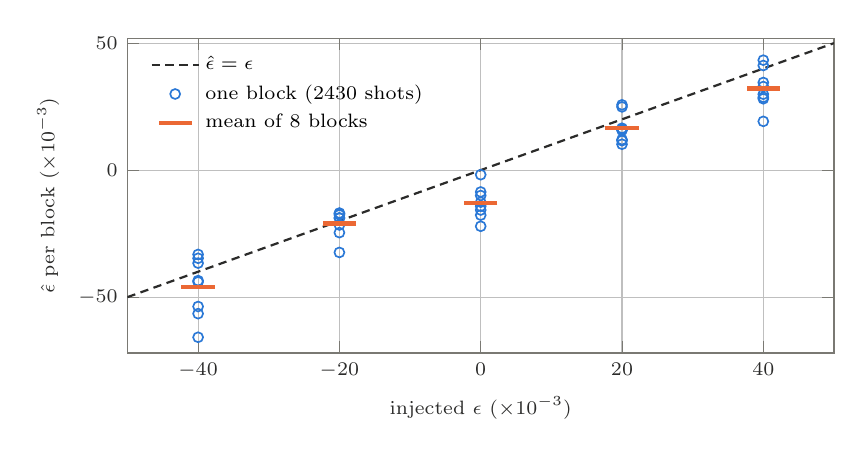
\begin{tikzpicture}
% Data: per-block epsilon_hat from followup/ibm-hardware-pilot/results/stage_a_postlock/analysis_corrected.json
% (identical to the locked per-block estimates in results/stage_a/analysis_primary.json). Units: 1e-3.
\begin{axis}[scaffold,scale only axis,width=0.74\columnwidth,height=4.0cm,xmin=-50,xmax=50,ymin=-72,ymax=52,
  xlabel={injected $\eps$ ($\times10^{-3}$)},ylabel={$\hat\eps$ per block ($\times10^{-3}$)},xtick={-40,-20,0,20,40},
  legend style={font=\scriptsize,draw=none,fill=none,at={(0.02,0.98)},anchor=north west,cells={anchor=west}}]
\addplot[ink,densely dashed,line width=0.8pt,domain=-50:50,samples=2] {x};
\addlegendentry{$\hat\eps=\eps$}
\addplot[only marks,mark=o,mark size=1.8pt,sN,line width=0.6pt] coordinates {
(0,-12.6)(0,-15.7)(0,-14.2)(0,-8.6)(0,-10.0)(0,-22.1)(0,-1.8)(0,-17.7)
(20,11.6)(20,25.7)(20,16.5)(20,12.0)(20,15.7)(20,10.2)(20,24.9)(20,16.0)
(-20,-16.9)(-20,-32.4)(-20,-21.6)(-20,-17.6)(-20,-17.1)(-20,-18.8)(-20,-24.6)(-20,-18.9)
(40,32.9)(40,28.7)(40,43.3)(40,41.2)(40,28.1)(40,19.2)(40,34.5)(40,29.9)
(-40,-36.6)(-40,-34.7)(-40,-33.2)(-40,-43.5)(-40,-65.8)(-40,-56.5)(-40,-53.7)(-40,-44.0)};
\addlegendentry{one block (2430 shots)}
\addplot[only marks,mark=-,mark size=6pt,sC,line width=1.6pt] coordinates {(0,-12.83)(20,16.58)(-20,-21.00)(40,32.21)(-40,-46.00)};
\addlegendentry{mean of 8 blocks}
\end{axis}
\end{tikzpicture}
\caption{HW-P1: P-amp estimates of the injected multiplicative error on \texttt{ibm\_marrakesh}. Each circle is one 2430-shot estimate; the bars are block means. The estimates track the injected value and flip sign correctly, but scatter by about $\pm0.008$ per estimate and are offset at zero injection ($-0.0128$). Hardware data, separate study; not a gate result.}
\label{fig:hw}
\end{figure}

\paragraph{Precision.} The spread of one 2430-shot estimate was $0.0053$--$0.0117$ across points and $0.0077$ pooled (95\% interval $0.0052$--$0.0084$), against the frozen threshold $0.0071429$: inconclusive at every point and pooled, with the pooled point estimate 8\% above the threshold. The pilot's locked analysis had divided this spread by $\sqrt8$, reporting the standard error of an eight-block mean instead, and labelled every point as meeting the threshold; an append-only erratum retracted those labels and added the corrected analysis (\cref{sec:repro}). With eight blocks the intervals are coarse, and the labels are descriptive.

\paragraph{Visibility and the synthetic margin.} The effective visibility, the mean amplitude $\sqrt{\langle X\rangle^2+\langle Y\rangle^2}$ over settings, was 0.948--0.957, well below the $0.99263$ at which the synthetic resource condition fails. Scaling the frozen conservative standard error $0.0070902$ by $1/v$ with $v=0.953$ gives $0.0074$, close to the observed $0.0077$ (a post-lock comparison): the hardware spread is about what the shot-noise model predicts once the measured contrast is included.

\paragraph{Accuracy.} The estimates track the injected values and change sign correctly, but they are biased. At zero injection the mean estimate was $-0.0128$ with 95\% interval $[-0.0166,-0.0086]$, which triggered the prespecified bias flag, and the additive phase was overestimated by $+0.0075$ to $+0.0094$ at every point. A native coherent phase on the qubit pair, for example from the CZ gate or a static $ZZ$ interaction, is a possible cause that the pilot did not test.

\subsection{What the pilot does and does not show}
The pilot shows that the idealisation behind Gate~1B does not hold on this processor: the measured contrast is far below the level the resource condition needs, the precision at the frozen budget is at best borderline, and the estimates carry an offset of about twice the precision threshold. An offset of that size is comparable to the errors the frozen grid injects ($|\eps|\le0.04$), so recalibrating with uncorrected P-amp estimates could itself add error; this was not tested. The pilot does not test correction, decisions, or the adaptive policy; it does not show that hardware has an angle-proportional error; and it covers one processor, one qubit pair, and one calibration window.

\section{Reproducibility and Errata}\label{sec:repro}

\paragraph{Append-only errata.} Frozen files are never edited. Nine errata correct the record: E001--E004 (one per gate), E005 (governance and environment), E006 (audit of the first erratum commit; Lemma~S1 narrowed, Lemma~B corrected, Gate~2 wording fixed), and E007--E009 (owner reviews of the identification lemmas, of the three-action results, and of S1$''$). Where errata differ, the later one governs. Errata files are hashed in six append-only manifests (\cref{tab:frozen} in \cref{app:tables}).

\paragraph{Internal recomputation.} A full recomputation (Linux x86-64, Python 3.13.18, NumPy 2.3.5) and a sampled one (every 50th unit; Python 3.10.12, NumPy 2.2.6) reproduce every verdict-level quantity, including Gate~3's $\DV$ and lower bound exactly. Stored per-unit floats differ in 416 of 6600 Gate~2 units and 31 of 5940 Gate~3/4 units, from last-bit platform differences in input probabilities that occasionally change one multinomial count; in every differing Gate~3 evaluation unit the change cancels inside $\Delta_u$. The original Python version and platform are unknown. This is internal recomputation, not independent validation.

\paragraph{Archive.} Release \texttt{v1.0.0-mt7-synthesis} (commit \texttt{66feb06}) is archived on Zenodo. The archive's SHA-256 and MD5 match the record, and its 119 files map one-to-one to the commit; 114 differ only in line endings.

\paragraph{Hardware pilot record.} The pilot's lock (canonical SHA-256 \texttt{f4b60e02\dots}) was committed before the first job; all eight submission and result receipts carry its hash, and the raw counts, IBM job identifiers, calibration snapshots, and the locked analysis output are hash-bound as post-run artifacts. Erratum HWP1-E001 records the precision-estimand error and its correction without altering any locked file; a dedicated check verifies the execution-time lock, the receipts, the locked artifacts, and that the corrected analysis reproduces from raw counts.

\paragraph{Checks and future locks.} The deterministic checks (errata and frozen-artifact manifests, archive metadata, RC and P-amp semantics, literature library, unit tests) run with the commands of \cref{tab:commands} and in continuous integration. Any future study must use the v2 lock template, which locks design files, every execution-code file, the environment, seeds, the exact command, absent outputs, and post-run artifact hashes together.

\section{Conclusion}\label{sec:conclusion}
\emph{When is runtime evidence sufficient to choose between trusting, correcting, and withholding a quantum decision under a fixed budget?} The theory gives the condition: the evidence must change the optimal action on a set of units large enough that the expected action-loss reduction exceeds the shots set aside for sensing and correction (\cref{prop:D1}); information-free policies never meet it (\cref{prop:P2}), and nearly dominated ones meet it only barely (P3). In the setting studied here the evidence was not sufficient. Retained randomized-compiling labels could not identify the multiplicative error at $\phi=0$ without knowledge of the ideal response; a known-reference sensor could, but its decision rule did not single out the units that benefit from correction; and because always correcting was already near-optimal, the adaptive policy had almost nothing to gain and showed no detectable value. These conclusions hold for the synthetic compiled-angle model and the frozen design. On a real processor the evidence was weaker still: with known errors injected, the sensor's precision at the frozen budget was inconclusive and its estimates were biased, so even the step that succeeded in simulation would need bias characterisation before any correction or policy could rely on it.

\section{Discussion}\label{sec:discussion}

\paragraph{What the negative results say.} Gate~1A does not say that randomized-compiling labels are uninformative: with a known response the oracle information is positive, and with known response directions the identified set is bounded. It says that an estimator that treats the response as unknown cannot recover $\eps$ at $\phi=0$. Gate~3 does not say that adaptive control is useless: in a model where always-correct is near-optimal, a policy built on a non-selective rule had little to gain, and the design---with estimated power 0.0004---could not have detected a small gain.

\paragraph{Limitations.} The error model is synthetic, the circuits have 2--6 qubits at QAOA depth one, and the simulation contains shot noise only; no gate result extends to visibility loss, decoherence, drift, context mismatch, structured nuisance models, larger circuits, or hardware. The P-amp resource condition fails for visibility below $0.99263$. Gate~2 lacked an uncertainty bound and power analysis, Gate~3 was underpowered, selection probabilities were Monte Carlo estimates, and the analysis code was outside the locks (\cref{sec:failure}). The Gate~3 estimand correction and the Gate~2 diagnostics are post-lock. Reproduction is internal and verdict-level, not bit-level across platforms (\cref{sec:repro}). The hardware pilot used injected errors, one processor, one qubit pair, one calibration window, and eight blocks; its precision correction is post-lock, and its approval was recorded after execution.

\paragraph{Next steps on hardware.} Before any decision study on hardware, the sensor's offset must be characterised and removed, for example by subtracting a zero-injection reference measured in the same block, and its precision established with more blocks than eight and on more than one qubit pair and calibration window. Only then would a decision-level stage that compares issuing and correcting under injected error be informative. A different question is whether the native fractional $R_{ZZ}(\theta)$ gate carries an angle-dependent coherent error of its own; that would be a characterisation study, and only a positive answer would give the compiled-angle model a physical carrier.

\paragraph{Further theory and design work.} A stronger test of adaptive control needs a model in which correction sometimes hurts, exact selection probabilities instead of Monte Carlo scoring, a power analysis committed before evaluation, and per-stratum comparators to close the metadata-only gap of \cref{prop:P2}.

\section*{Data and code availability}
All frozen artifacts, errata, audit tools, and proofs are in the repository and in the Zenodo archive (version DOI 10.5281/zenodo.24443391; concept DOI 10.5281/zenodo.24443390). The hardware pilot's protocol, lock, raw counts, IBM job identifiers, calibration snapshots, and corrected analysis are in the repository under \texttt{followup/ibm-hardware-pilot/}; they postdate that archived version. The repository is public for inspection and citation under the terms in \texttt{RIGHTS.md}; it is not open-source licensed.

\bibliographystyle{abbrv}
\bibliography{references}

\clearpage
\onecolumn
\appendix

\section{Proofs of the three-action results}\label{app:theory}

Throughout, \cref{ass:X,ass:pol,ass:st2} hold. All action-conditional losses are measurable in $x$ (regular conditional laws exist on standard Borel spaces) and take values in $[0,\max(1,\lA,\lF)]$, so every expectation is finite. These proofs follow the owner-reviewed note \texttt{docs/theory/A4\_A6\_rigorous.pdf}; \cref{lem:TVup} and \cref{app:estimand} are new and carry the status \textsc{proved, draft}.

\paragraph{Proof of \cref{thm:T1}.} Fix $\vt$ and condition on $X=x$. The realised loss is
$L=\one\{a=N\}\one\{\delta_0\neq k^*\}+\one\{a=A\}\lA+\one\{a=C\}[\lF F+(1-F)\one\{\delta_C\neq k^*\}]$.
Since $a=\alpha(x,U)$ and $U$ is independent of $Y=(F,\delta_C)$ given $X=x$,
$\E[\one\{a=C\}(\lF F+(1-F)\one\{\delta_C\neq k^*\})\mid X=x]=\pi_C(x)\,(\lF\rho+c)=\pi_C(x)l_C(\vt,x)$.
The N and A terms equal $\pi_N(x)l_N(\vt,x)$ and $\pi_A(x)\lA$ because $l_N$ is a function of $x$. Taking $\E_\vt$ (tower property; bounded terms) gives \eqref{eq:T1a}; substituting $\pi_N=1-\pi_C-\pi_A$ gives \eqref{eq:T1b}. The three summands of $L$ are indicators of the disjoint events ``issued and wrong'', ``abstain'', ``C and fail'' (weighted by $1,\lA,\lF$), so $R=P(\text{issue}\wedge\text{wrong})+\lA P(A)+\lF P(C\wedge F{=}1)$. Without \cref{ass:st2} (e.g.\ a policy that peeks at a preliminary corrected shot) the C term fails. \hfill\qedsymbol

\paragraph{Proof of \cref{cor:C1}.} With $\pi_C\equiv0$, $\lA=0$, $\pi_A=\one_{\mathrm{Alarm}}$, \eqref{eq:T1b} gives $R=q_f+\E[\one_{\mathrm{Alarm}}(0-\one_{W_f})]=q_f-d_f$; then $R<q_0\iff d_f>q_f-q_0$. \hfill\qedsymbol

\paragraph{Proof of \cref{cor:C2}.} Average \eqref{eq:T1b} over $\Pi$; by the tower property $\E[\pi_A(X)l_N(\vt,X)]=\E[\pi_A(X)e_N(X)]$, so the Bayes risk is $r(\pi)=\E[e_N(X)]+\E[\pi_A(X)(\lA-e_N(X))]$. Pointwise, $\pi_A(x)(\lA-e_N(x))\ge\min\{0,\lA-e_N(x)\}$ with equality iff $\pi_A(x)=1$ when $e_N(x)>\lA$ and $\pi_A(x)=0$ when $e_N(x)<\lA$. The stated policy is measurable and attains the pointwise minimum; any other policy is strictly worse unless it agrees a.e.\ off the tie set. \hfill\qedsymbol

\paragraph{Proof of \cref{prop:P1} and P3.} By \eqref{eq:T1a} and the tower property, the Bayes risk of $\pi$ is $\E[\sum_a\pi_a(X)\rho_a(X)]$, minimised pointwise by any $a\in\arg\min_a\rho_a(x)$; the pairwise conditions are $\rho_a<\rho_b$ written out. $\mathrm{VOI}_{\mathrm{alloc}}$ is the Bayes risk of always-$a_0$ minus that of the Bayes policy; its integrand $\rho_{a_0}-\min_a\rho_a$ is non-negative and vanishes a.s.\ iff $a_0$ is Bayes a.s. \emph{P3}: if $\rho_a\le\rho_b$ for every $b$ and a.e.\ $x$, always-$a$ attains the pointwise minimum, so it is Bayes and $\mathrm{VOI}_{\mathrm{alloc}}=0$. \hfill\qedsymbol

\paragraph{Proof of \cref{lem:L1}.} Both regrets integrate against the same $P$ with the same weights:
$\Reg(\pi;\vt)+\Reg(\pi;\vt')=\E_P[\sum_a\pi_a(X)(D_a(\vt,X)+D_a(\vt',X))]\ge\E_P[\Gamma(X)]$, since a convex combination is at least its minimum. The maximum is at least half the sum. Because $D\ge0$, $\Gamma(x)=0$ iff some $a$ has $D_a(\vt,x)=D_a(\vt',x)=0$. Wrong-action form: $P_{\vt'}(a\neq a_1)\ge P_{\vt'}(a=a_0)=\E_P[\pi_{a_0}(X)]=P_\vt(a=a_0)=1-P_\vt(a\neq a_0)$; no optimality hypothesis is used. \hfill\qedsymbol

\paragraph{Proof of \cref{thm:T2}.} (T2a) $\Reg_0+\Reg_1=\int\sum_a\pi_a(D^0_ap_0+D^1_ap_1)\,d\mu\ge\int\sum_a\pi_a(D^0_a+D^1_a)\min(p_0,p_1)\,d\mu\ge\int\Gamma\min(p_0,p_1)\,d\mu$. The $\Gamma_{\min}$ form follows from $\int\min(p_0,p_1)=1-\TV$. (T2c) $P_0(a\neq a_0)+P_1(a=a_0)=\int[(1-\pi_{a_0})p_0+\pi_{a_0}p_1]\ge\int\min(p_0,p_1)$, and $P_1(a\neq a_1)\ge P_1(a=a_0)$. (T2e, Le Cam) $\sqrt{p_0p_1}=\sqrt{\min(p_0,p_1)\max(p_0,p_1)}$, so by Cauchy--Schwarz $\BC^2\le\int\min\int\max=(1-\TV)(1+\TV)\le2(1-\TV)$. (T2d, Bretagnolle--Huber) If $\KL(P_0\|P_1)<\infty$ then $P_0\ll P_1$, $Z=\sqrt{p_1/p_0}>0$ $P_0$-a.s.\ and $\BC=\E_{P_0}Z$; Jensen for the concave logarithm gives $\log\BC\ge\E_{P_0}\log Z=-\tfrac12\KL(P_0\|P_1)$, and Le Cam gives $1-\TV\ge\tfrac12\BC^2\ge\tfrac12e^{-\KL}$. $\BC$ and $\TV$ are symmetric, so the same holds with $\KL(P_1\|P_0)$. For independent coordinates, Fubini gives $\BC(P_0^{\otimes},P_1^{\otimes})=\prod_i\BC_i$ and $\KL=\sum_i\KL_i$. \hfill\qedsymbol

\begin{lemma}[TV--Bhattacharyya upper bound]\label{lem:TVup}\status{proved, draft}
For any $P,Q$ with densities $p,q$, $\TV(P,Q)\le\sqrt{1-\BC(P,Q)^2}$. For product laws, $\TV(P^{\otimes n},Q^{\otimes n})\le\sqrt{1-\BC_1^{2n}}$.
\end{lemma}
\begin{proof}
$2\TV=\int|p-q|=\int|\sqrt p-\sqrt q|(\sqrt p+\sqrt q)\le\bigl(\int(\sqrt p-\sqrt q)^2\bigr)^{1/2}\bigl(\int(\sqrt p+\sqrt q)^2\bigr)^{1/2}=\sqrt{(2-2\BC)(2+2\BC)}=2\sqrt{1-\BC^2}$ by Cauchy--Schwarz. The product statement follows from $\BC_n=\BC_1^n$.
\end{proof}
\noindent This is the inequality used by \texttt{tools/audit\_gate1a\_pairs\_budget.py} for its stored upper bound on $\TV_n$; the tighter two-point bound in \cref{sec:ident} is $(1-\sqrt{1-\BC_n^2})/2$.

\paragraph{Proof of \cref{prop:D1}.} Averaging \eqref{eq:T1b} over $\Pi$ and using \cref{ass:comp}(a), $\E_\Pi q(\vt)=\bar q_f$, so $\bar R(\pi)=\bar q_f-G(\pi)$ and $R_{\mathrm{fix}}-\bar R=G-(\bar q_f-R_{\mathrm{fix}})$; $K\ge0$ because $R_{\mathrm{fix}}\le\bar q_f$. \hfill\qedsymbol

\paragraph{Proof of \cref{prop:P2}.} By \eqref{eq:T1a} with constant weights, $R(\pi;\vt)=w_N\E_\vt l_N+w_C\E_\vt l_C+w_A\lA$. Averaging, $\bar R(\pi)=w_N\bar q_f+w_C\bar r_C+w_A\lA$, where $\E_\Pi\E_\vt l_C=\bar r_C$ by \cref{ass:comp}(b) and \eqref{eq:T1a} for the always-C policy. If $w_C>0$, (b) guarantees $\bar r_C$ is a comparator. Each of $\bar q_f$, $\bar r_C$, $\lA$ is $\ge R_{\mathrm{fix}}$, so their convex combination is too. Equality holds iff each action with $w_a>0$ has risk exactly $R_{\mathrm{fix}}$. \hfill\qedsymbol

\section{Proofs of the identification results and Lemma B}\label{app:ident}

These follow the owner-reviewed notes \texttt{docs/theory/S1prime\_B\_rigorous.pdf} and \texttt{S1doubleprime\_rigorous.pdf}. Observed draws are $(c,t,b)$ with law $Q(c,t,b)=w_c\pi_c(t)P_{c,t}(b)$ and known $w_c,\pi_c(t)>0$; candidate and outcome sets are finite.

\paragraph{\Cref{thm:S1}(1).} Let $m=\min_{c,b}q^0_c(b)>0$ (a finite minimum of positive numbers), $V=\max_c\|v_c\|_\infty$, and $\delta=m/V$ ($\infty$ if $V=0$). For $|\eps'-\eps_0|<\delta$ define $q'_c=q^0_c+(\eps_0-\eps')v_c$, $D'=D^0$, $\phi'=0$. It sums to one since $v_c\in\Sigma_0$. If $v_c(b)=0$ then $q'_c(b)=q^0_c(b)>0$; otherwise $|(\eps_0-\eps')v_c(b)|<\delta V=m\le q^0_c(b)$. For every $t$, $P'_{c,t}=q'_c+\eps'v_c=q^0_c+\eps_0v_c=P_c\in\simp$, so the point is admissible in N-q and, with $D'=D^0$, in N-loc. \hfill\qedsymbol

\paragraph{\Cref{prop:sharp}.} Let $(\eps',\phi',q')$ be equivalent to the truth. For the candidate in the hypothesis, $P'_{c,t}-P'_{c,t'}=\phi'\sum_\ell(s_\ell(t)-s_\ell(t'))D^0_{c\ell}$ must vanish for all $t,t'$, forcing $\phi'=0$. Then $q'_c=q^0_c-(\eps'-\eps_0)v_c$ for every $c$, and the only remaining constraint is positivity, $q^0_c(b)-(\eps'-\eps_0)v_c(b)>0$ for all $c,b$, i.e.\ $-\alpha<\eps'-\eps_0<\beta$. A non-zero $v_c\in\Sigma_0$ has entries of both signs, so both minima are over non-empty sets. Note $\delta=m/V\le\min(\alpha,\beta)$. \hfill\qedsymbol

\paragraph{\Cref{thm:S1}(2).} Let $\eps'\in\R$, $\phi'=0$. If $\eps'\neq0$: $D'_{c\ell}=(\eps_0/\eps')D^0_{c\ell}$, $q'_c=q^0_c$, so $\eps'v'_c=\eps_0v_c$ and $P'_{c,t}=P_c$. If $\eps'=0$: $q'_c=P_c$, $D'=0$. Both points are admissible. \hfill\qedsymbol

\paragraph{\Cref{thm:S1}(3).} Let $\eps'\in\R$ and $R'_c(u)=R^0_c(u+(\eps_0-\eps')\theta_c)$, $\phi'=0$. By (F1) $R'_c$ is in the class, maps into $\simp$, and has the regularity of $R^0_c$. By \cref{lem:frame}, $P'_{c,t}=R'_c((1+\eps')\theta_c)=R^0_c((1+\eps_0)\theta_c)=P_c$ for every $t$. No restriction $1+\eps'\neq0$ is needed. \hfill\qedsymbol

\paragraph{\Cref{thm:S1}(4).} Every score has the form $\dot P_{c,t}(b)/P_{c,t}(b)$, a bounded function since all $P_{c,t}(b)>0$. \emph{Score for $\eps$:} under N-q/N-loc $\partial_\eps P_{c,t}=v_c$; under N-free, by the chain rule at $\phi=0$, $\partial_\eps R_c((1+\eps)\theta_c+s(t)\phi)=\nabla R_c(u^0_c)\theta_c=:w_c$. Neither depends on $t$, and $v_c,w_c\in\Sigma_0$. \emph{Nuisance path with the same score:} under N-q/N-loc, $q^\tau_c=q^0_c+\tau v_c$ stays in the class for $|\tau|<m/V$ and has score $v_c/P_c$. Under N-free, $R_c$ is continuous at $u^0_c$, so $\min_bR_c(u)(b)\ge m_c/2$ on a ball around $u^0_c$ ($m_c=\min_bP_c(b)$); with a $C^\infty$ bump $\psi_c\in[0,1]$, $\psi_c(u^0_c)=1$, supported in that ball, $R^\tau_c=R_c+\tau\psi_cw_c$ sums to one, is positive for $|\tau|<m_c/(2\|w_c\|_\infty)$, lies in the class by (F2), and has score $w_c/P_c$. So the $\eps$-score lies in the nuisance tangent set; its projection onto the orthocomplement of the closed linear span is $0$ and the efficient information is $0$. Enlarging the nuisance (e.g.\ $\phi$ unknown) only enlarges the tangent set. \hfill\qedsymbol

\paragraph{\Cref{cor:gibbs}.} Let $\Lambda(\eps',\phi',\eta')=\sum_cw_c\sum_t\pi_c(t)\sum_bP_{c,t}(b)\log P'_{c,t}(b)$ and $\Lambda^*$ the same with $P'=P$. Then $\Lambda^*-\Lambda=\sum_cw_c\sum_t\pi_c(t)\KL(P_{c,t}\|P'_{c,t})\ge0$, with equality iff $P'=P$. Hence $\sup_{\phi',\eta'}\Lambda(\eps',\cdot)=\Lambda^*$ is attained iff $\eps'\in I$. If the true laws are only label-invariant and in $\simp$ (not of N-q form), the choice $q'_c=P_c-\eps'v_c$, $\phi'=0$ still attains $\Lambda^*$ for $\eps'$ in an open interval around $0$. \hfill\qedsymbol

\paragraph{S1$''$.} One context, candidates $k=1,\dots,K$ with angle vectors $\Theta_k$, one map $R$, $P_{k,t}=R((1+\eps)\Theta_k+s(t)\phi)$, truth $\phi_0=0$, $1+\eps_0\neq0$.
(a) If the class is closed under $R\mapsto R(c\,\cdot)$, $c\neq0$: for $\eps'\neq-1$ put $c=(1+\eps_0)/(1+\eps')$, $R'=R(c\,\cdot)$, $\phi'=0$; then $P'_{k,t}=R((1+\eps_0)\Theta_k)=P_k$.
(b) If $(-1,\phi',R')$ is equivalent, then $P'_{k,t}=R'(s(t)\phi')$ does not depend on $k$ for any fixed $t$ and any $\phi'$, so all $P_k$ coincide; conversely $R'\equiv P_1$ works if they do.
(c) First-order shared: $P_{k,t}=q+\sum_\ell(\eps\Theta_{k\ell}+s_\ell(t)\phi)D_\ell$; for $\eps'\neq0$, $D'=(\eps_0/\eps')D$, $q'=q$, $\phi'=0$; at $\eps'=0$ the law $q'+\phi'\sum_\ell s_\ell(t)D'_\ell$ does not depend on $k$, so $0\in I$ iff all $P_k$ coincide.
(d) Monotonicity: if every point of $M$ has an image in $M''$ with the same laws, identified sets in $M''$ contain those in $M$; laws $vP+(1-v)o$ with $v\in(0,1]$ contain the original class at $v=1$.
In each of the six primary designs at each $\phi_0=0$ grid point, $I$ contains an open interval around $\eps_0$ realised with $\phi'=0$, so it meets the box $[-0.05,0.05]^2$ in a non-degenerate interval. \hfill\qedsymbol

\paragraph{\Cref{thm:B}.} \emph{Step 0.} Each entry of $\RZ(x)$ is $\cos(x/2)$ or $\pm i\sin(x/2)$, so $E_j$ is a polynomial in $\{\cos(x_{ji}/2),\sin(x_{ji}/2)\}$ and $g\in C^\infty$. \emph{Step 1.} Fix all coordinates but $x=x_{ji}$; $U_j=V_2\RZ^{(k)}(x)V_1$ and $\langle b|U_j|{+}^n\rangle=\cos\tfrac x2\alpha_b-i\sin\tfrac x2\beta_b$, so $E_j=a+b\cos x+c\sin x$ with $a=\tfrac12\sum_bs(b)(|\alpha_b|^2+|\beta_b|^2)$, $b=\tfrac12\sum_bs(b)(|\alpha_b|^2-|\beta_b|^2)$, $c=-\sum_bs(b)\,\mathrm{Im}(\alpha_b\bar\beta_b)$. \emph{Step 2.} If $f=a+b\cos x+c\sin x\in[0,1]$ on $\R$ and $\rho=\sqrt{b^2+c^2}>0$, then $f=a+\rho\cos(x-x_0)$, $a+\rho\le1$, $a-\rho\ge0$, so $\rho\le\tfrac12$ and $|f'|\le\tfrac12$. Since $E_j=\sum_bs(b)p(b)\in[0,1]$ for every unitary, $|\partial E_j/\partial x_{ji}|\le\tfrac12$ everywhere. \emph{Step 3.} $x_A,x_B$ are disjoint coordinates, so $\|\nabla g\|_\infty\le\tfrac12$ on $\R^M$, and $|g(\theta+\delta)-g(\theta)|=|\int_0^1\nabla g(\theta+t\delta)\cdot\delta\,dt|\le\tfrac12\|\delta\|_1$ by Hölder. \emph{Step 4.} $|\delta_{ji}|\le|\eps||\theta_{ji}|+|\phi|$; summing gives $\|\delta\|_1\le|\eps|A+|\phi|M$. \emph{Sharpness:} one qubit, $W_0=I$, $W_1=H$, $s(0)=1$, $s(1)=0$ give $E=\cos^2(x/2)$ and the ratio tends to $1$ as $\delta\to0$ at $x=\pi/2$. \emph{Companion bound:} $|\Delta g|\le\min(\tfrac12\|\delta_A\|_1,1)+\min(\tfrac12\|\delta_B\|_1,1)$. \hfill\qedsymbol

\section{Gate 3 estimands}\label{app:estimand}

\begin{proposition}[Frozen-estimand bias]\label{prop:cov}\status{proved, draft}
Fix a unit. Let $W$ be the event that $\delta_0$ is wrong, $q=P(W)$, and $N$ the event that the policy chooses N, both functions of the same stage-1 shots. The frozen N-path contribution $\E[\one_N]\,q$ and the conditional contribution $\E[\one_N\one_W]$ satisfy
$\E[\one_N]q-\E[\one_N\one_W]=-\mathrm{Cov}(\one_N,\one_W)$.
Averaged over units, with the comparator and the C and A losses unchanged, $\DV^{\mathrm{frozen}}=\DV^{\mathrm{corrected}}+\overline{\mathrm{Cov}(\one_N,\one_W)}$, up to Monte Carlo error in the stored estimate of $q$; a non-positive average covariance therefore makes the frozen $\DV$ the smaller of the two.
\end{proposition}
\begin{proof}
$\E[\one_N]q-\E[\one_N\one_W]=P(N)P(W)-P(N\cap W)=-\mathrm{Cov}(\one_N,\one_W)$. In $\Delta_u=L_{\mathrm{fixed},u}-L_{\mathrm{policy},u}$ only the N-path term of $L_{\mathrm{policy},u}$ changes, entering with a minus sign.
\end{proof}
\noindent In the stored records (\emph{deterministic recomputation}): mean N-path loss on the 919 N units is $0.00278$ (frozen) and $0.00218$ (realised); contributions to $\DV$ by action are N $-0.000260$, C $0$, A $+0.000340$ (frozen) and N $-0.000104$, C $0$, A $+0.000340$ (corrected). The corrected column uses the realised indicator of the single realised initial run, as in \texttt{tools/audit\_gate34\_estimand.py}. Only the N-path term changes; the A contribution is the same in both columns ($0.0003405$).

\section{Tables}\label{app:tables}

\begin{table}[h]
\centering\small
\caption{Evidence classes and proof-status labels used in the paper.}\label{tab:labels}
\begin{tabularx}{\textwidth}{@{}>{\raggedright\arraybackslash}p{4.6cm}X@{}}
\toprule
Label & Meaning \\
\midrule
analytic & a mathematical result within the stated model; its proof status is one of the next five rows \\
proved (owner-reviewed) & complete proof checked line by line by the author; recorded in errata E007--E009; the default in the main text, not tagged \\
proved, draft & complete proof written for this paper and not yet independently reviewed; tagged where it appears \\
conditional & a result whose premise is not proved; tagged \\
specification inference & a step that depends on the wording of a frozen specification rather than on mathematics; tagged \\
open & an unresolved question; tagged \\
numerical check & exact or floating-point evaluation of instances; never a proof \\
simulated (gate output) & produced by a gate run under its lock: shot-noise-only simulation of the compiled-angle model; the default for empirical numbers \\
post-lock & an analysis specified after the gate result; may qualify a verdict, cannot change it \\
recomputed & arithmetic on stored per-unit fields, done for this paper \\
internal recomputation & re-running the project's code on another platform; not third-party validation \\
hardware (HW-P1) & counts from IBM hardware in the separately locked pilot of \cref{sec:hardware}; never enters a gate verdict \\
\bottomrule
\end{tabularx}
\end{table}


\begin{table}[h]
\centering\small
\caption{Notation.}\label{tab:notation}
\begin{tabularx}{\textwidth}{@{}>{\raggedright\arraybackslash}p{5.2cm}X@{}}
\toprule
Symbol & Meaning \\
\midrule
$u=(G,c,\nu,r)$ & evaluation unit: graph, candidate pair, noise condition, replicate \\
$\vt=(r_{\mathrm{ideal}},\eps,\phi,\eta)$ & latent state; $k^*(\vt)$ the correct candidate; $g=\mu_A-\mu_B$ the ideal gap \\
$\eps,\phi$ & multiplicative and additive coherent error: $\RZ(a)\mapsto\RZ((1+\eps)a+\phi)$ \\
$s_\ell(t)\in\{\pm1\}$ & label sign of tagged rotation $\ell$ under label pattern $t$ \\
$N,C,A$ & issue, recalibrate-and-rerun, abstain \\
$N=24{,}300$; $n_S,n_{T0},n_C$ & total budget; sensor, initial-target, and reserve shots ($2430$, $10{,}934$, $10{,}936$) \\
$\lA,\lF$ & abstention and correction-failure losses ($1/4$) \\
$X=(m,X_S,X_{T0})$ & stage-1 evidence; $\delta_0$, $\delta_C$ issued answers on N and C \\
$l_N,l_C,l_A$ & action-conditional losses; $e_N$ posterior wrong-answer probability; $\rho_a$ posterior action risks \\
$\Reg$, $D_a$, $\Gamma$ & regret, action excess loss, pairwise minimum excess loss \\
$\TV,\BC,H^2,\KL$ & total variation $\tfrac12\int|p-q|$; Bhattacharyya $\int\sqrt{pq}$; Hellinger $\int(\sqrt p-\sqrt q)^2=2-2\BC$; Kullback--Leibler \\
$\bar q_0,\bar q_f,\bar r_C,R_{\mathrm{fix}}$ & comparator population risks and their minimum \\
$\DV$, $G$, $K$ & primary endpoint; action-loss reduction; allocation cost \\
N-q, N-loc, N-free & nuisance classes (known directions; unknown affine response; free response) \\
$I$ & identified set for $\eps$ \\
$A,M$ & $\sum|\theta_{ji}|$ and number of tagged rotations; $B=|\eps|A+|\phi|M$, $\hat B$ its plug-in \\
\bottomrule
\end{tabularx}
\end{table}

\begin{table}[h]
\centering\small
\caption{Gate~1A hard pairs at $n_S=2430$ under the oracle law. Columns 3--6 are from \fn{results/errata/gate1a_pairs_at_budget.json} (post-lock, E001 §4); the last column is $(1-\TV_n^{\mathrm{ub}})/2$ (deterministic recomputation). Action relevance is nonevaluable: no action map was frozen.}\label{tab:pairs}
\begin{tabular}{@{}llrrrrr@{}}
\toprule
Context & $(\theta_{\mathrm{ref}},\eps_1)$ & $\KL_n$ & $\BC_n$ & $\TV_n$ upper bound & error $\ge$ (Le Cam/BH) & error $\ge$ (\cref{lem:TVup}) \\
\midrule
G2 & $(\pi/8,+0.02)$ & 0.150 & 0.9632 & 0.2687 & 0.2319 & 0.3656 \\
G2 & $(\pi/8,-0.02)$ & 0.150 & 0.9632 & 0.2687 & 0.2319 & 0.3656 \\
G2 & $(\pi/4,+0.02)$ & 0.606 & 0.8608 & 0.5089 & 0.1852 & 0.2455 \\
G2 & $(\pi/4,-0.02)$ & 0.594 & 0.8608 & 0.5089 & 0.1852 & 0.2455 \\
G3 & $(\pi/8,+0.02)$ & 0.280 & 0.9326 & 0.3608 & 0.2174 & 0.3196 \\
G3 & $(\pi/8,-0.02)$ & 0.279 & 0.9323 & 0.3616 & 0.2173 & 0.3192 \\
G3 & $(\pi/4,+0.02)$ & 0.514 & 0.8800 & 0.4749 & 0.1936 & 0.2625 \\
G3 & $(\pi/4,-0.02)$ & 0.575 & 0.8650 & 0.5017 & 0.1871 & 0.2491 \\
\bottomrule
\end{tabular}
\end{table}

\begin{table}[h]
\centering\small
\caption{Frozen result, governing erratum, and living interpretation.}\label{tab:frozen}
\begin{tabularx}{\textwidth}{@{}l>{\raggedright\arraybackslash}X>{\raggedright\arraybackslash}X>{\raggedright\arraybackslash}X@{}}
\toprule
Gate & Frozen record (unchanged) & Erratum & Current interpretation \\
\midrule
1A & FAIL; I3, recovery, controls hard-coded & E001, E006 §2, E007, E009 & FAIL on the basis of \cref{thm:S1}, \cref{cor:gibbs}, S1$''$ and spec §7/§9 (specification inference) \\
1B & PASS & E002 & PASS in the noiseless known-reference model; 0.74\% margin; fails for $v<0.99263$ \\
2 & PASS & E003, E006 §4 & formal PASS; not evidence of useful benefit selection (authoritative wording) \\
3 & FAIL ($\DV=0.0000804$, LB $-0.000743$) & E004 & FAIL; corrected post-lock estimand also FAIL ($0.000237$, $-0.000625$); power $0.0004$ \\
4 & PASS & E004 §4 & PASS, moot; thresholds not power-derived \\
all & locks of design documents & E005, E006 §7 & code outside locks; future studies use lock template v2 \\
HW-P1 & locked analysis labelled all five points ``meets'' & HWP1-E001 & labels retracted; single-estimate precision inconclusive at every point and pooled ($0.0077$ vs $0.0071429$); zero-injection bias flagged \\
\bottomrule
\end{tabularx}
\end{table}

\begin{table}[h]
\centering\small
\caption{Theorem-to-evidence crosswalk. ``Ledger'' refers to \fn{docs/claim_ledger.md}.}\label{tab:thm}
\begin{tabularx}{\textwidth}{@{}>{\raggedright\arraybackslash}p{4.6cm}>{\raggedright\arraybackslash}p{3.6cm}>{\raggedright\arraybackslash}X l@{}}
\toprule
Result & Status & Proof location & Ledger \\
\midrule
Frame covariance (\cref{lem:frame}) & proved, owner-reviewed & \fn{S1prime_B_rigorous.pdf} Lemma 2; \cref{sec:model} & A1, A2 \\
T1, C1, C2 & proved, owner-reviewed & \fn{A4_A6_rigorous.pdf} §2; \cref{app:theory} & A4 \\
P1, P3 & proved, draft & theory note §3, §6; \cref{app:theory} & --- \\
L1, wrong-action form, T2 & proved, owner-reviewed & \fn{A4_A6_rigorous.pdf} §3; \cref{app:theory} & A5 \\
\Cref{lem:TVup} (TV upper bound) & proved, draft & \cref{app:theory} & --- \\
Example E1 (corrected) / E2 & proved / conditional, open & E008 §2--3; \cref{ex:E1,ex:E2} & A5 \\
D1, P2 & proved, owner-reviewed & \fn{A4_A6_rigorous.pdf} §4; \cref{app:theory} & A6 \\
Lemma S1$'$ (1)--(4), \cref{prop:sharp}, \cref{cor:gibbs} & proved, owner-reviewed & \fn{S1prime_B_rigorous.pdf}; \cref{app:ident} & A3 \\
S1$''$ (a)--(d) & proved, owner-reviewed & \fn{S1doubleprime_rigorous.pdf}; \cref{app:ident} & A3 \\
Non-uniqueness $\Rightarrow$ FAIL & specification inference & E007 §3.1 & B1 \\
Readings exhaust spec §5.3 & open & E007 §3.2, E009 & B1 \\
Lemma B (\cref{thm:B}) & proved, owner-reviewed; numerical check $0.431$/$0.213$ & \fn{S1prime_B_rigorous.pdf} §4; \cref{app:ident} & A7 \\
Frozen-estimand bias (\cref{prop:cov}) & proved, draft & \cref{app:estimand} & B5 \\
\bottomrule
\end{tabularx}
\end{table}

\begin{table}[h]
\centering\small
\caption{Claim-to-evidence crosswalk for every empirical statement.}\label{tab:claims}
\begin{tabularx}{\textwidth}{@{}>{\raggedright\arraybackslash}p{3.8cm}>{\raggedright\arraybackslash}X>{\raggedright\arraybackslash}p{3.4cm}>{\raggedright\arraybackslash}p{4.4cm}@{}}
\toprule
Claim & Value & Evidence class & Source \\
\midrule
Gate 1A zero efficient info at $\phi=0$ & $\le6.8\times10^{-21}$/shot; oracle $0.24$--$0.62$ & post-lock numerical check & \fn{gate1a_efficient_information.json} \\
Gate 1A two-point error at budget & $\ge0.185$ (Le Cam/BH); $\ge0.245$ (\cref{lem:TVup}) & post-lock; deterministic recomputation & \fn{gate1a_pairs_at_budget.json} \\
Gate 1B identification & rank 2; 81/81 within $10^{-8}$ & frozen (noiseless simulation) & \fn{gate1b_results.json} \\
P-amp semantics & 729 cases, max dev.\ $3.4\times10^{-15}$ & post-lock deterministic check & \fn{check_pamp_semantics.py} \\
Gate 1B margin & $0.74\%$; fails for $v<0.99263$ & frozen + arithmetic & \fn{gate1b_results.json}, E002 \\
Gate 2 verdict & BA $0.5871$ vs $0.5$; LOGO min $0.0658$ & frozen (shot-noise simulation) & \fn{gate2_results.json} \\
Gate 2 selectivity & precision $0.093$ vs base $0.077$; decomposition & post-lock, exploratory & \fn{gate2_diagnostics.json} \\
Gate 2 P2 blindness & 3300 of 6600 units & post-lock deterministic check & E003 §5 \\
Gate 3 verdict & $\DV=0.0000804$, LB $-0.000743$ & frozen (shot-noise simulation) & \fn{gate34_results.json} \\
Gate 3 corrected estimand & $0.000237$, LB $-0.000625$ & post-lock reanalysis & \fn{gate34_estimand.json} \\
Gate 3 decomposition & N $-0.000260$, A $+0.000340$ & deterministic recomputation & \fn{gate34_results.json} units \\
Power & $0.0004$; MDM $0.000665$ & frozen (same run as evaluation) & \fn{power_analysis.md} \\
Gate 4 & N 25.9\%, C 72.6\%, A 1.5\% & frozen & \fn{gate34_results.json} \\
Lemma B ratio & max $0.431$ / $0.213$ & post-lock numerical check & \fn{gap_shift_bound_check.json} \\
Reproducibility & 416/6600, 31/5940 float diffs; verdicts identical & internal recomputation & \fn{reproducibility_full.json}, E005 \\
HW-P1 precision & pooled SD $0.0077$ $[0.0052,0.0084]$; inconclusive & hardware; post-lock correction & \fn{followup/ibm-hardware-pilot/results/stage_a_postlock/analysis_corrected.json} \\
HW-P1 bias, visibility & $\eps$ bias $-0.0128$ at zero; $v=0.948$--$0.957$ & hardware; locked analysis & \fn{followup/ibm-hardware-pilot/results/stage_a/analysis_primary.json} \\
\bottomrule
\end{tabularx}
\end{table}

\begin{table}[h]
\centering\small
\caption{What may and may not be said.}\label{tab:say}
\begin{tabularx}{\textwidth}{@{}>{\raggedright\arraybackslash}X>{\raggedright\arraybackslash}X@{}}
\toprule
Supported (with stated scope) & Not supported \\
\midrule
In the synthetic model, a deployable estimator treating the response as unknown cannot recover $\eps$ from retained labels at $\phi=0$ (Gate~1A FAIL). & ``RC labels cannot sense $\eps$'' in general, on hardware, or under structured nuisance models (oracle information is positive). \\
Zero efficient information, local non-identification (all classes), global non-identification (N-loc, N-free), bounded identified set (N-q). & Global non-identification inferred from zero Fisher information. \\
P-amp identifies $(\eps,\phi)$ from its own known reference, noiselessly, with a 0.7\% margin. & P-amp robustness, P-amp superiority over P2, or hardware transfer. \\
Gate~2 formal PASS with the authoritative qualification. & ``Gate~2 predicts correction benefit'' or ``shows decision relevance'' without the qualification. \\
No detectable net value over always-correct; power $0.0004$. & ``The method works'' or any positive policy value. \\
Lemma B: global, exact population bound on the expected gap shift. & That $\hat B$ guarantees a decision-flip bound or has coverage. \\
Internal recomputation reproduces every verdict. & ``Validated'', ``independently reproduced'', ``third-party verified'', ``preregistered'', ``first''. \\
HW-P1: with injected errors, P-amp precision at 2430 shots was inconclusive against the threshold; estimates were biased; visibility 0.95. & ``P-amp met its precision threshold on hardware''; ``hardware validates the method''; ``hardware has the modelled error''; HW-P1 ``preregistered''. \\
\bottomrule
\end{tabularx}
\end{table}

\begin{table}[h]
\centering\small
\caption{Artifact map and reproducibility commands. Run from the repository root.}\label{tab:commands}
\begin{tabularx}{\textwidth}{@{}>{\raggedright\arraybackslash}p{7.7cm}X@{}}
\toprule
Path or command & Content or check \\
\midrule
\fn{docs/contracts/decision_problem_v1.md} & decision contract, D1--D3 (M3-locked) \\
\texttt{docs/theory/*.tex, *.pdf} & owner-reviewed proofs (S1$'$/B, A4--A6, S1$''$) and review drafts \\
\fn{docs/freeze/}, \fn{docs/theory/gate1_math_spec_v1.md} & gate design locks and manifests \\
\texttt{results/\{gate1a,gate1b,dev,gate34\}/} & frozen gate artifacts \\
\fn{docs/errata/}, \fn{results/errata/} & errata E001--E009, audit outputs, manifests v1--v6 \\
\fn{docs/claim_ledger.md}, \fn{docs/results/project_status.md} & claim ledger and living status \\
\texttt{python -m unittest discover -s tests} & unit tests (or \texttt{python -m pytest -q tests}) \\
\texttt{python tools/check\_errata\_artifacts.py} & errata manifests and every frozen lock/artifact check \\
\texttt{python tools/check\_archive\_manifest.py} & archive identifiers agree across documents \\
\texttt{python tools/check\_hwp1\_postlock.py} & HW-P1 execution lock, receipts, locked artifacts, and corrected analysis \\
\texttt{python tools/check\_hwp1\_postlock.py} & HW-P1 execution lock, receipts, locked artifacts, and corrected analysis \\
\texttt{python tools/check\_rc\_semantics.py} & 64 RC label--angle equivalence cases \\
\texttt{python tools/check\_pamp\_semantics.py} & 729 P-amp circuit cases against the phase model \\
\texttt{python tools/check\_library.py} & literature library structure \\
\texttt{python tools/audit\_gate34\_estimand.py} & frozen Gate~3 numbers, then the corrected estimand \\
\texttt{python tools/audit\_reproducibility.py 50} & sampled recomputation of Gate~2 and Gate~3/4 units \\
\texttt{python tools/build\_technical\_report.py} & compiles this paper from its LaTeX source \\
\bottomrule
\end{tabularx}
\end{table}

\end{document}
